\documentclass[11pt,a4paper]{article}

%--------------------
% Packages
% -------------------
\usepackage[utf8x]{inputenc}
\usepackage{CormorantGaramond}
\usepackage{orcidlink}
\usepackage[english]{babel}
\usepackage[natbib=true,backend=biber,sorting=nyt,style=apa]{biblatex}
\addbibresource{LaTeX/citations/ba_thesis_citations.bib}
\usepackage[a4paper, lmargin=0.1666\paperwidth, rmargin=0.1666\paperwidth, tmargin=0.1111\paperheight, bmargin=0.1111\paperheight]{geometry}
\usepackage{fancyhdr}
\renewcommand{\baselinestretch}{1.35}
\usepackage[flushleft]{threeparttable}
\usepackage{amsmath}
\usepackage[capposition=top]{floatrow}
\usepackage{makecell}
\usepackage{graphics}
\usepackage{rotating}
\usepackage{multicol}
\usepackage{breakurl}
\usepackage[all]{nowidow}



% Doument setup
\hypersetup{
    colorlinks=true,
    urlcolor=blue,
    linkcolor=black,
    citecolor=black
}
\setlength{\parindent}{4em}
\setlength{\parskip}{1em}
\setlength{\skip\footins}{2pc plus 5pt minus 2pt}
\frenchspacing

\fancyhf{}
\fancyhead[L]{\textbf{UZH – Department of Political Science}}
\fancyhead[R]{Bachelor's thesis – V3 20240429}
\fancyfoot[L]{Timothy Justin Oesch}
\fancyfoot[R]{\thepage}
\renewcommand\headrulewidth{0pt}
\pagestyle{fancy}

\usepackage{etoolbox}
\AtBeginEnvironment{quote}{\par\singlespacing\small}

%Footnote definition
\makeatletter 
\renewcommand{\@makefntext}[1]{
    \setlength{\parindent}{0pt}
    \begin{list}{}{
    \setlength{\labelwidth}{1.5em}
    \setlength{\leftmargin}{\labelwidth}
    \setlength{\labelsep}{3pt}
    \setlength{\itemsep}{5pt}
    \setlength{\parsep}{0pt}
    \setlength{\topsep}{0pt}
    \footnotesize}
    \item[\@makefnmark\hfil]#1
    \end{list}
}
\makeatother

\begin{document}
\begin{titlepage}
\title{
    \raggedright
    \small
    \textsc{Bachelor's Thesis} \\
    \vspace{0.5cm}
    \fontsize{25pt}{25pt}
    \textbf{Playing Moneyball}\\
    \vspace{0.2cm}
    \Large\textit{Analyzing the influence of election campaign budgets on the media agenda and electoral outcomes} \\
    
    \vspace{1cm}

    \textbf{Timothy Justin Oesch \orcidlink{0000-0002-4302-5086}}\\
    \vspace{0.25cm}
    \normalsize
    \textbf{Student ID:} 18-719-187\\
    \textbf{Address:} Agnesstrasse 42, CH-8004 Zürich\\
    \textbf{E-mail:} \href{mailto:timothyjustin.oesch@uzh.ch}{\underline{timothyjustin.oesch@uzh.ch}}\\
    
    \vspace{0.5cm} 
    Written in the seminar\\
    \textit{«Agenda-settig: How do issues get important?»}\\
    Module ID: 24FS/23HS 615-BAa
    
    \vspace{0.5cm}
    Written under the supervision of\\
    \textbf{Dr. Jonathan Klüser PhD}

    
    
    \vspace{0.25cm}
    \scriptsize{
        Word count: XXXXXXX \\
        Submission date: June 1, 2024
    } \\
    
    \date{}
    \begin{figure}[b]
        \centering
        \includegraphics[width=200px]{LaTeX/partials/01.1_uzh_logo.png}
    \end{figure}
}
\clearpage\maketitle
\thispagestyle{empty}
\end{titlepage}

\newpage
\pagestyle{fancy}
\pagenumbering{gobble}
\tableofcontents

\newpage

\listoffigures
\listoftables

\newpage

\pagenumbering{roman}

\begin{abstract}
    Amet aliquam id diam maecenas ultricies mi eget. Fringilla phasellus faucibus scelerisque eleifend donec pretium vulputate sapien nec. Lectus urna duis convallis convallis. Sem et tortor consequat id porta nibh venenatis cras sed. Ultricies tristique nulla aliquet enim tortor at auctor. Feugiat pretium nibh ipsum consequat nisl vel pretium lectus. Ac feugiat sed lectus vestibulum mattis ullamcorper. Felis donec et odio pellentesque diam volutpat commodo. Aliquam sem et tortor consequat id porta nibh venenatis cras. Sed enim ut sem viverra aliquet. Vel quam elementum pulvinar etiam non quam. Feugiat pretium nibh ipsum consequat nisl vel pretium lectus. Ac feugiat sed lectus vestibulum mattis ullamcorper. Felis donec et odio pellentesque diam volutpat commodo. Aliquam sem et tortor consequat id porta nibh venenatis cras. Sed enim ut sem viverra aliquet. Vel quam elementum pulvinar etiam non quam.
\end{abstract}

\section*{Introduction: A well-known puzzle.}
\addcontentsline{toc}{section}{\protect\numberline{}Introduction: A well-known puzzle.}

One of the few times the general public gets into contact with political scientists is during election season and on election days: Pundits, experts and analysts all try to explain why a campaigning party or individual is behaving in a certain way and, when the deed is done, they will contextualize the results, predict the consequences of the electoral outcomes and, in light of surprising results, try to decipher which factors were causal for the loss of a sure-set winner or the win of an underdog. This last question, linking supply- and demand-side components, institutional factors and the political landscape to the vote tally, is one of political science’s most interesting and most pressing questions: \textit{Which characteristics contribute to a party’s electoral success? Which contribute to its demise?} A plethora of studies and papers have tried to find answers to these conundrums and yet, electoral surprises are a dime a dozen: Be it the defeat of Hillary Clinton in the 2016 presidential election, Jeremy Corbin’s Labour party exceeding everyone’s expectations in Theresa May’s failed snap election in 2017, or the incredible victory of the \textit{CHP} in Turkey in the country’s most recent local elections. At the time of writing this introduction, exactly 7 days have passed since a gargantuan shift in Turkey’s political landscape took place. In a major upset, the opposition party around Istanbul’s mayor Ekrem İmamoğlu has enjoyed a landslide victory and was able to dethrone Erdoğan’s \textit{AKP} as the outright winner of any national election since the \textit{AKP}’s establishment in 2001: The \textit{CHP }was able to flip 9 constituencies from Erdoğan’s party, leading the BBC to title \textit{«Opposition stuns Erdogan with historic victory»} (\cite{kirby_turkish_2024}) , quoting president Erdoğan himself as saying that the outcome marked \textit{«a turning point»}. The Foreign Policy Magazine announced that \textit{«Post-Erdogan Turkey Is Finally Here»} (\cite{cook_post-erdogan_2024}), while the Swiss \textit{Tages-Anzeiger} proclaimed that \textit{«Sunday marked the beginning of the end of Erdogan»} (\cite{geiger_kommentar_2024}). All these cases clearly show that there is much to learn about the inner workings of election outcomes.

In typical Swiss fashion, such crass election swings seem far from realistic in Switzerland; while the outcomes of direct-democratic referenda are at times more unexpected (as a recent example, one can think of the acceptance of a 13\textsuperscript{th} yearly retirement payment by Swiss voters), a system where \textit{«Konkordanz»}\footnote{In simple terms the idea that a large supermajority of parties ought to be represented in governmental decision-making.} is king will inherently lead to more stable election results. The power and potential consequences of elections are therefore easily forgotten.

Party elites are nonetheless eager to investigate how results came to be: When listening to elites and party activists alike, especially among the political left, it seems to be a popular grievance that, since their opponents’ investments into rallying efforts felt substantially larger than their own, their adversaries were able to reach more voters and reach them better. Such explications make intuitive sense: Spend more, get a larger audience. Past research has acknowledged the prevalence of popular beliefs linking campaign funds to electoral outcomes (\cite{scott_money_2015, sorauf_inside_1992}). As a campaigner and aspiring political scientist myself, I have made the baffling experience that the widespread and undisputed conviction among the general public that financial resources are a central, if not \textit{the} central, factor in determining political success, the state of the sciences is inconclusive. Questions surrounding the effects of campaign funds seem to be another example of where popular belief and scientific evidence diverge.

Another prevalent argument surrounds what I would like to call the \textit{«larger political climate»}: It is evidently important that, for a party to succeed, voters will need to know what a party stands for on the one hand, and on the other, they will need to perceive the issues a party highlights to be relevant. Loosing parties will often argue that they were unable to talk about what was \textit{«on people’s minds»} and they were therefore unable to rally support and mobilize beyond their party’s base. This suggestion touches upon two relevant subjects: \textit{Issue salience} and the \textit{public agenda}. Past literature has held ample debate around how topical importance\footnote{The terms \textit{«importance»}, \textit{«centrality»}, \textit{«ego-involvement»}, and \textit{«salience»} have all been used to describe a concept that is, to the extent of this paper, essentially identical and they will be used interchangeably. For a more nuanced definition, see Krosnick (\citeyear{krosnick_role_1988}).} shapes a voter’s preferences and there is evidence in favor of the hypothesis that more important issues will have stronger impacts on a voter’s choices (\cite{krosnick_role_1988, krosnick_government_1990}). Embedding this idea into the research of the analysis hereinafter allows us to ask the question at heart of the field of agenda setting: How do topics become important? More specifically: \textit{Why do people perceive an issue to be the most important one?}

The following pages shall suggest a path forward: Through analysis of the applicable literature, I will propose a mechanism in the field of electoral research that unifies considerations surrounding campaign funds and their effects on the \textit{«political climate»}. This mechanism allows me to stipulate three hypotheses revolving around the nexus of campaign activity and party budgets, its ramifications on firstly the quantitative representation of parties in the media and secondly the substantive topics represented in the media agenda. Put simply: I set out to test whether campaign budgets influence how active a party can be during the election period, which could in turn change how often they appear and how successfully they can situate their issues in the media. I will go on to argue what the consequences of these hypotheses, if true, would be. A novel dataset and the use of an automated coding process of media articles and party programs allows me to test these hypotheses against the backdrop of a recent Swiss election, concluding in summarizing the broader scientific implications of this thesis and highlighting its shortcomings and future research potential.


\newpage
\pagenumbering{arabic}
\section{A trident of knowledge: Relevant scientific literature }
Before digging into the pertinent literature, let me mark off which scientific foundation this thesis is resting on. My approach shall resemble a trident: The first point considers how agenda setting processes shape the way vote choices come into existence. I will thereunto zoom in on the relevance of issue-salience and how it shapes a voter’s perception of electoral options. Moving closer to the key subject of this paper, I will scrutinize the conjunction of topic relevance and the media. The second point will discuss, if and how political actors are trying to influence the media agenda. The third and last point shall scrutinize the current state of campaign budget research, highlighting nuances in a diffuse debate. 

\subsection{The first prong: Does issue-salience matter?}
\subsubsection{Chasing causality: A brief outline.}
As it would amount to hubris to claim this thesis could summarize a field of research as tremendously large as the one concerned with explaining vote choices, I will rely on the summarizing work by \citeauthor{kulachai_factors_2023} (\citeyear{kulachai_factors_2023}). The authors group the mechanisms they identified into three sections: Individual-level, socio-cultural and political explanations. 

While the individual-level reasonings include socioeconomic/-demographic elements (age, gender, education and income) and intrapersonal factors (political ideology, personality traits and emotional intelligence), I want to highlight the fact that \citeauthor{kulachai_factors_2023} group two political issues into these explanations: \textit{«Healthcare Experiences»} and \textit{«Climate Change Concerns»}. I want to argue the notability of this by emphasizing that in both cases, the authors attach voting behavior to the mechanisms through the issue’s salience: Whereas the COVID-19 pandemic put topics surrounding the healthcare system in the limelight and the \textit{«urgency of addressing climate change has become increasingly salient among voters»}, these two subjects have become overarching determinants of voting behavior. The second and third group of rationalizations in the article include a potpourri of cultural and political factors, of which I will address a few in the following subchapters.

\subsubsection{Honing in on issue salience.}
As the likely most significant study – and arguably the most comprehensive case against the impact of issue positions and salience on vote choices – \citeauthor{kulachai_factors_2023} mention \textit{«The American voter» }(\cite{campbell_american_1960}). In this influential seminal study, the authors popularized the Michiganian view of vote choices where partisan identification is far and beyond the strongest predictor of electoral behavior. Yet, I want to call the validity of this theory for the analysis at hand into question: Firstly, the case is heavily centered around the American political system and questionably applicable in other contexts, and secondly there has been significant scientific opposition, exemplified by Key’s infamous quote that \textit{«voters are not fools»} (\cite{key_responsible_1966}).

In his \citeyear{krosnick_role_1988} paper, Krosnick reassesses the arguments in the domain of issue salience and their impact on vote choices and delivers a mechanism in which this effect might manifest itself. He finds evidence that the centrality voters assign to issues does potently determine how they evaluate candidates and their voting behavior. Krosnick proposes that this is a result of the fact that more important issues are more readily available in voters’ memories, and they seem to be able to differentiate candidates more easily on these topics. In 1990, he states further that voters’ salient attitudes are highly resistant to change (\cite{krosnick_government_1990}).

Fournier et al. (\citeyear{fournier_issue_2003}) expand on Krosnick’s work by linking issue importance to governmental performance evaluations (another popular determinant of voting behavior) and – for this paper more importantly – through a theoretical discussion of problem salience in the domain of agenda-setting. The authors contest that the array of topics that voters will use to evaluate electoral options is not all encompassing. They posit that, due to \textit{«human cognitive limitations»}, voters will inevitably focus on the evidence that comes to their minds easily and quickly. The fundament of these considerations can be found in the book section by Miller and Krosnick (\citeyear{miller_news_1996}): The authors paint voters’ attitudes as a network of mental nodes with a relative strength which is determined by how frequently that node has been activated: \textit{«The more one has thought about an attitude in the past, the stronger its node will be»}. Subsequently, the stronger a node, the more readily available its information will be and, in accordance with Fournier et al., the more influential it will be when casting a vote. Delineating from traditional persuasion, where factors influence the substantive position voters hold, agenda-setting and priming are the processes where actors influence said node-strength.

\subsubsection{The forth estate and its powers: Linking issue-salience to the media.}
Taking the next step in this endeavor, it is now time to turn to who these actors are. Using an at the time innovatory experimental setting, Iyengar and Kinder (\citeyear{iyengar_news_1987}) deliver indubitable evidence to how the news media influences political priorities. By unrecognizably altering news broadcasts, adding stories concerned with either national security or unemployment into their midst and presenting two groups of volunteers with one of the versions, they were able to show that subjects exposed to more national security content were more likely to rate national security as a higher political priority and vice versa. 

They thereby lay credence to Cohen’s claim that the media \textit{«may not be successful much of the time in telling people what to think, but it is stunningly successful in telling its readers what to think about»} (\cite{cohen_press_1964}). These experiments and the four studies in Miller and Krosnick (\citeyear{miller_news_1996}) strongly support the framework proposed by McCombs and Shaw: In their paper, they make a succinct case that the electorate does turn to mass media for political information. They analyze the agenda setting function of mass media in-depth, finding a substantial correlation between the foci of the mass media and the public at large. While the authors were hesitant about their findings, the context provided in the years since the study’s publication lead me to contend that, indeed, \textit{«voters do learn»} (\cite{mccombs_agenda-setting_1972}).


\subsubsection{Summary and implications}
Before examining the ways in which political actors will try to influence the media, I shall briefly recap the submitted knowledge so far and its implications for this paper: The literature shows that issue salience is a significant determinant of voting behavior and delivers a cognitive causal pathway. Papers by Krosnick et al. and Fournier et al. provide mechanisms in which salience is determined by agenda-setting processes and priming effects. Lastly, the publications by Iyengar and Kinder and Miller and Krosnick revealed – in laboratory as well as natural survey settings – that media actors significantly influence which topics become central in voters’ minds and which don’t. The significance of these findings cannot be overstated: While the general reader might already hold the belief that the news media shapes our political landscape profoundly – or as Schudson (\citeyear{schudson_news_1988}) put it in his review of Iyengar and Kinder: \textit{«Why should it take fourteen laboratory experiments in Ann Arbor and New Haven, involving more than l ,000 participants from all walks of life, conducted over a four-year period from 1980 through 1983, to demonstrate the obvious?»} – providing omnifarious and indubitable scientific evidence for this commonsense belief is one of the cornerstones of my analysis. 


\subsection{The second prong: Do politicians matter?}
The second and third part in this review of the scientific literature are more narrowly circumscribed but I’d argue just as important as the first one. I will now turn to the question: \textit{What does the state of the sciences say about political actors’ influence on the media agenda?} 


\subsubsection{Are we human or are we dancer?}
I want to argue this conundrum through two opposing camps in line with the distinction proposed by Beckett (\citeyear{beckett_setting_1994}): In her paper, Beckett analyzes how the «Street crime»-issue became part of the public agenda, identifying the \textit{objectivist model} and the \textit{constructionist model }as possible explanations. Proponents of the objectivist account argue that a social problem, i.e. phenomena that influence social well-being (\cite{manis_concept_1974}), will become a part of the political discourse largely independently from subjective interference. In this narrative, impartial cognizance of the situation around an societal state is a \textit{«necessary and largely sufficient condition for the identification of a social problem.»} In addition, objectivists posit that political action is a result of reactionary problem solving as opposed to proactive shaping of public opinion. Constructionists set forth the idea that, in order for social conditions to become part of the public interest, reality must be interpreted through the use of frames (\cite{hall_policing_1978}). They believe that an abundance of actors compete for which of these frames will become part of the political hegemony (\cite{edelman_constructing_1988,gamson_media_1992}) by drawing attention to specific aspects of the problem they are advocating for. 

Beckett goes on to differentiate between \textit{culturalist} and \textit{elite constructionism}. While this distinction might seem pedantic, it is, I’d argue, at the heart of the mechanism I am proposing: While culturalist-constructionists agree with the framing-principle, thereby disagreeing with objectivists on the root causes of why an issue becomes part of the agenda, they still see political action as the result of public opinion. Elite-constructionists on the other hand propose that political elites – facilitated by the news media’s need for credible or \textit{«institutional»} sources – will be the ones who get the ball rolling, or as Bennett (\cite{bennett_public_1980}) puts it: \textit{«[…] the general public is most often called on by interest groups and elites to participate in the debate about issues that have already been defined.»} This means that in an elite-constructionist world, political activity is not the consequence, but the cause of public opinion. Beckett, notably, also calls this distinction a «pluralist v. agenda-setting» discussion.

Beckett goes on to test 4 hypotheses, providing significant evidence in favor of the agenda-setting, constructionist account. In summary, the assumption that her findings are independent of the specific social topic implies that it is political and media elites who will shape the public agenda. Conversely, Wasow (\citeyear{wasow_agenda_2020}) acknowledges that the scientific consensus gathers around a constructivist worldview, but proclaims the debate over elite- or culturalist constructivism unresolved even more than 2 decades after Beckett’s paper.

\subsubsection{Political activity and the media.}
For the purpose of this paper, I will abstain from debating this point, incorporating elite-constructionism as a premise of my framework. In the concluding remarks, I will discuss the consequences if this conjecture is erroneous and suggest a solution for future research. I believe it to be more fruitful to ask not \textit{if} elites influence the media but \textit{how} they would do such a thing. Presuming that campaigning parties deem it necessary to get voters to think about issues at the core of their program, also referred to as \textit{owning issues}\footnote{For a description on issue ownership, see Petrocik (\citeyear{petrocik_issue_1996}) and Stubager (\citeyear{stubager_what_2018}).}, they will invest their campaign resources accordingly. It makes intuitive sense that, in order to get in front of as many eyes and into as many minds as possible, campaigners will among other things use the amplifying effects of traditional media outlets. Drawing on research in the field of media studies, Patro et al. (\citeyear{patro_characterizing_2018}) describe how universities will use widespread tendencies in the human psyche by exaggerating scientific findings for their publications to gain traction in the media, finding that half the press releases of specific universities employ such strategies. For the lack of this kind of scrutiny in the field of political communication, I would instead argue that if even universities – citadels of integrity as they claim to be – (ab)use our innate human affinity for sensational claims, actors running for office are not likely to refrain from doing so. The broader illations of this assumption will become clear once we turn to specifying the mechanism and operationalizing campaign activity in the respective chapters.


\subsection{The third prong: Does money matter?}
Before proceeding to answer the titular query of this part, I want to ask a meta question: \textit{Why does it matter if money matters?} Let’s assume that there was scientific consensus in favor of a causal link between financial ability and electoral success: If that was the case, I argue it would be reasonable to urge lawmakers to pass a regulatory framework governing \textit{who} is allowed to spend \textit{how much} money \textit{within which ruleset}. The subjunctive formulation attests to the fact that, in Jeffrey Milyo’s words, the study of campaign finance is \textit{«more notable for its faults and oversights than for its contributions»} (\cite{milyo_political_1999}). In my point of view, this is one of the reasons why countries such as Switzerland have yet to adopt comprehensive laws governing campaign finances. This chapter will try to give a brief rundown of publications in favor and against an etiological linkage of gold and gain and make a case for why further research will be justified even if all arrows point to no connection.

\subsubsection{Standing on vertigo-inducing shoulders: Inconclusive evidence about money in politics.}
I would be remiss if I did not mention the extraordinary works of Gary Jacobs and Peverill Squire: Their publications expertly summarize the field’s findings (\cite{jacobson_money_1985,squire_candidates_1995}). While both authors focus exclusively on US-elections, I see no reason why the findings they present would not be able to serve as guiding principles. One significant argument is, that if we are able to explain voting behavior through campaign-detached factors, most prominently the state of the economy, there is no room left for campaigns to make a difference. Past research has made conflicting findings on whether economic performance sufficiently determines electoral outcomes,\footnote{In favor: Born (\citeyear{born_strategic_1986}); Carson \& Jacobson (\citeyear{carson_politics_2024}); Lewis-Beck \& Rice (\citeyear{lewis-beck_forecasting_1992}), against: Alesina \& Rosenthal (\citeyear{alesina_partisan_1989}); J. E. Campbell (\citeyear{campbell_presidential_1997}); Erikson (\citeyear{erikson_economic_1990}).} notably being unable to port aggregate-level findings to the individual level.

To reconcile these difficulties, studies have resorted to investigating the effects of which information voters \textit{have access to}, \textit{retain} and \textit{utilize} to make a decision. The argument summarized in Converse (1962) proclaims the existence of a \textit{floating voter}: An individual with little information and involvement, susceptible to changing their preferences based on campaign activity. Yet again, the derived hypotheses are hotly debated. Zaller (\citeyear{zaller_bringing_1989}) qualifies the theory, introducing the notion of \textit{«differential information flow»}, finding that different levels of campaign intensity and voters’ prior partisan attachment can lead diverse voter groups to be influenced by campaign activity.

The last point I want to shed light upon is the discussion whether regulating campaign finances – the practical implication of any study of money in politics – is justified in its own right. As multiple authors have pointed out, the restriction of spending can be thought of as a restriction on free-speech rights (\cite{kang_end_2012,ortiz_democratic_1998}) and as such must follow the ideas of necessity, proportionality and suitability. Cordis and Milyo (\citeyear{cordis_state_2013}) and Milyo (\citeyear{milyo_state_2012}) have analyzed if limiting funds has reduced public corruption and increased public trust in government respectively, both finding no significant relation, calling the suitability of such measures into question.\footnote{Notably, it is unclear if the 2012 paper was subject to peer-review as it was published on the Social Science Research Network SSRN. Similarly note-worthy is the provenance of the 2013 study, as it was published under the patronage of George Mason University, an institution that was widely criticized for accepting significant financial support by conservative billionaires like Charles Koch (\cite{larimer_george_2018}).} Fouirnaies and Fowler (\citeyear{fouirnaies_campaign_2022}) showed that, in general, financial contributions of the insurance industry have little effect on public policy, leading one to challenge the necessity of campaign finance laws. Since proportionality is subject to interpretation and both necessity and suitability of campaign finance regulation seem to be questionable, the case against campaign finance regulation is likely strong. In light of recent events, one could argue: \textit{If the glove don’t fit, you must acquit}.


\subsubsection{Empiricism over morality: Bridging a gap.}
Having completed this brief treatise on the relevance of financial campaign resources, it is now time to approach a superordinate dillemma: Jeffrey Milyo (\citeyear{milyo_political_1999,milyo_state_2012}) argues that \textit{«no collective decision rule can always satisfy a certain reasonable set of “rationality” conditions»}. In his \citeyear{scott_money_2015} paper, he goes so far as to say that because \textit{«democratic processes cannot be expected to produce policies that are rational or just»}, it is unreasonable to discuss the question of how money influences politics against the backdrop of morality or justice. Although the validity of this morally nihilist argument might seem dubious, Milyo argues that the question on campaign finance regulation must take place in an empirical setting. Hertig (\citeyear{hertig_sind_1982}) analyzes the influence of campaign budgets on Swiss direct democratic votes and finds heavy skewedness of campaign resources between political camps. In opposition of Milyo’s belief, he concludes:
\begin{quote}
\textit{[...] but even if we were to overestimate the potential and actual effect of pure voting propaganda on the decision-making of voters, the identified advertising structure is still reason enough to critically question the balance of power that prevails in the formation of opinion prior to votes.\footnote{ Hertig is using voting propaganda as a proxy for campaign budgets, an established best practice for the Swiss case, since concrete financial data has been lacking until today. Translated from German, see the original text (p.56) for literal quote.}}
\end{quote}
In his monograph, Sorauf (\citeyear{sorauf_inside_1992}) reviews the situation of campaign finance regulations in the US of the time, concluding in two chapters where he proposes several ways forward for campaign finance reform. One striking element of these last two chapters are his stands on the influence of \textit{political action committees} (PACs): He claims that, since there is no evidence linking «PAC-money» to outcomes regarding public policy, there is not enough reason to ban or even just limit these forms of political organization. In a tough-but-fair review of his work, Gross (\citeyear{gross_inside_1993}) calls this the «Burden of Proof Question», highlighting that Sorauf places this burden on the individuals trying to reform campaign finance law. Gross emphasizes that there are \textit{«different and disproportionately important consequences of placing the burden of proof in the wrong place»}. Gross concedes that \textit{«one typically works on the assumption that the burden of proof is on those trying to establish a relationship»}, but because of the immense complexity of finding empirical evidence for the influence of PAC-money and the fatal consequences of falsely assuming there to be no connection, it is reasonable to put the burden-of-proof on those arguing against campaign finance restriction. In a time where the courts, established in \textit{Citizens United v. Federal Election Commission} (\citeyear{kennedy_citizens_2010}) and \textit{SpeechNOW.org v. Federal Election Commission} (\citeyear{sentelle_speechnoworg_2010}), have essentially allowed so called «super PACs» to raise and spend a practically unlimited amount of money\footnote{ As long as they do not coordinate with stakeholders such as candidates they are supporting, a fact that has become a practical joke in popular culture.} in the US based on free speech considerations, one can only wonder if Frank Sorauf would still believe in his position as he passed away only 3 years after the decisions were published.

This is the exact context in which this study takes place; the crossroads between empirical observations and questions of morality, ethics, and justice. It is the prescribed goal of the analysis to test whether there is a so far missed link between campaign spending and electoral outcomes through the means of issue-salience and, therefore, regulations for campaign finance are justified, not just when scrutinizing them philosophically, but also empirically.


\section{Framework and empirical implications}

\subsection{The case for a new model.}

\subsubsection{Making Money Moves: Three steps from cash to conversation.}
The model set out to be tested can be stylized as depicted in Figure 1. \textit{Campaign funds} are connected to a \textit{party’s resources} intuitively: The more money a party can invest into an election campaign, the more people that party can engage professionally, the larger their ad-buy, the more resources they have at their disposal to do communication research, content creation, activist mobilization and more. This leads the party to be a more potent influence on the agenda-setting process through \textit{campaign activity}. 

\begin{figure}[htbp]
    \centering
    \includegraphics[width=1\linewidth]{LaTeX/figures/Process.png}
    \caption{Proposed mechanism linking campaign funds to the public agenda through campaign activity.}
    \label{fig:enter-label}
\end{figure}
The next step, connecting the agenda-setting process to the \textit{media and public agenda}, is grounded in two premises: Firstly, political elites are assumed to want to be \textit{«as relevant as possible»}, meaning they want to make their parties and their issues visible. In my view, subscribing to this idea in line with the principle of rational utility-maximizing actors is in this case unproblematic. Secondly – as noted and justified above – the mechanism relies on the concept that the public agenda is shaped by \textit{elite-constructivism}, meaning that voters turn to the media to make sense of the world around them (hence constructivism) and the media takes cues from political elites to decide which issues to highlight in their reporting (hence elitism). The crux in this presumption lies not in the constructivist but the elitist aspect, a dispute which this paper will not be able to weigh in on. But even if one believes in a more pluralist worldview, there is room for an alternative mechanism: Such reflections can be incorporated in the position that the more money a party has, the more easily they can \textit{conform to} the public discussion rather than set the public agenda.\footnote{ In the conclusion to this paper, I am proposing a way in which this analysis could be amended in order to lay credence to an elitist pathway.}

The last portrayed step from the public agenda to the electoral result is an implicit one: As shown above, the scientific debate around the influence of issue salience on vote choice is far from settled. Even though this paper does not aim to add to this controversy directly, I find it relevant to keep an eye on the bigger picture and suggest that future research traces the machinery I proposed all the way to electoral outcomes, as this is where the most practical implications in regards to policymaking lie.


\subsubsection{Putting flesh on the bone: Hypotheses.}
I am now ready to propose three hypotheses that can be derived from my framework.
\textit{The agency hypothesis (H1):} My framework suggests that the higher a campaign’s resources, the larger their campaign output to set the public agenda. My first hypothesis should therefore read: \textit{The higher a party’s election campaign budget, the more active they are during an election campaign.}

\textit{The frequency hypothesis (H2):} The second implication of my model is, that campaigning parties want to be as salient as possible in the time leading up to an election in order to be atop voters’ minds. In order to achieve this, they will try to appear in the media as frequently as possible. The second hypothesis I therefore present goes: \textit{The higher a party’s election campaign budget, the more frequently they will appear in media reporting.}

\textit{The issue salience hypothesis (H3):} The third and final derivative I take away from my machinery surrounds the centrality of issues in the media agenda. If parties are competing for the issues they put at the forefront of their program to take up space in the media and campaign activity has an effect on the news’ content, then there should be a correlation between campaign budgets and media issue salience. This leads me to claim: \textit{The higher a party’s election campaign budget, the more likely it is that the issues that are relevant for them are relevant in the media agenda as well.}

\subsection{Empirical implications: What should we observe?}
Before moving on to test these claims, I will here delimit which observations would underpin them. Support for H1 would be if the quantity of campaign activity rose in tandem with campaign budgets. In other words: It would aid H1 if parties are campaigning more vigorously when they have higher budgets. For H2 to be validated, we would need to see an analog rise in party occurrence in media reporting correlating with campaign budgets. While the expected evidence for H1 and H2 is rather intuitive, H3 is a harder nut to crack: For me to establish a relationship between campaign budgets and issue salience in the media, I propose to analyze the effect of the interaction between issue salience for a party and that party’s campaign budget on the salience of the issue in the media. Put simply: The best evidence for H3 is, if the topics important to a party with a high campaign budget are more salient in the media than the topics important to a party with a low campaign budget.


\section{Empirical analysis}

\subsection{Case selection}
As previously hinted to, my analysis surrounds the Swiss national elections of 2023 for the larger chamber of parliament. This case is suitable in several regards: Firstly, there is novel data available for the campaign funding. For the first time in Swiss history, all parties and interest groups were obligated to transparently provide how much money they fundraised during the election and which candidates benefited from it. Secondly, Switzerland is the only member state of the Council of Europe to have practically no restrictions on political financing (\cite{jaberg_largent_2019}): Such restrictions could skew our analysis. Lastly, the key-metrics of average swing and turnout were nominal for the 2023 election as shown in \autoref{tab:tab1} and \autoref{tab:tab2}: The average party-swing was at around 1\%, while turnout was at 46.6\%.


\begin{table}
    \begin{threeparttable}
        \centering
        \caption{Swing calculations for the Swiss federal elections from 1999–2023.}
        \vspace{0.5cm}
        \label{tab:tab1}
        \begin{tabular*}{\linewidth}{@{\extracolsep{\fill}} | l | l | l | l | l | l | l | l | }
            \hline
            \textit{Party}\textbf{ / Year} & \textbf{2023} & \textbf{2019} & \textbf{2015} & \textbf{2011} & \textbf{2007} & \textbf{2003} & \textbf{1999} \\
            \hline
            \textit{SVP} & +2.3\% & –3.8\% & +2.8\% & –2.4\% & +2.2\% & +4.2\% & +7.7\% \\
            \hline
            \textit{SP} & +1.5\% & –2.0\% & +0.1\% & –0.9\% & -3.7\% & +0.8\% & +0.7\% \\
            \hline
            \textit{FDP} & –0.8\% & –1.3\% & +1.3\% & –2.5\% & -1.5\% & -2.6\% & -0.4\% \\
            \hline
            \textit{Mitte} & +0.2\% &   &   &   &   &   &   \\
            \hline
            \textit{Grüne} & –3.4\% & +6.1\% & –1.3\% & –1.2\% & +2.2\% & +2.3\% & -0.2\% \\
            \hline
            \textit{glp} & –0.2\% & +3.2\% & –0.8\% & +4.0\% & +1.4\% &   &   \\
            \hline
            \textit{EVP} & –0.1\% & +0.2\% & –0.1\% & –0.4\% & +0.1\% & +0.5\% & +/-0\% \\
            \hline
            \textit{EDU} & +0.2\% & –0. 2\% & –0.1\% & +/-0\% & +/-0\% & +/-0\% &   \\
            \hline
            \textit{CVP} &   & –0.2\% & –0.7\% & -2.2\% & +0.1\% & -1.4\% & -1\% \\
            \hline
            \textit{BDP} &   & –1.6\% & –1.3\% & +5.4\% &   &   &   \\
            \hline
            \textit{LPS} &   &   &   &   & -0.4\% & -0.1\% & -0.4\% \\
            \hline
            \textit{SD} &   &   &   &   &   & -0.8\% & -1.3\% \\
            \hline
            \textit{other} & +0.3\% & –0.3\% & +0.1\% & +0.2\% & -0.4\% & -3\% & -2\% \\
            \hline
            \textbf{Average Swing} & \textbf{1.00\%} & \textbf{1.89\%} & \textbf{0.86\%} & \textbf{1.92\%} & \textbf{1.2\%} & \textbf{1.57\%} & \textbf{1.68\%} \\
            \hline
        
        \end{tabular*}
        \begin{tablenotes}
            \footnotesize
            \item \textit{Note: 24-year-average swing of 1.45\%, 24-year-median swing of 1.57\%.}
        \end{tablenotes}
    \end{threeparttable}
\end{table}


\begin{table}
    \begin{threeparttable}
        \centering
        \caption{Turnout statistics for the Swiss federal general elections from 1999–2023.}
        \vspace{0.5cm}
        \label{tab:tab2}
        \begin{tabular*}{\linewidth}{@{\extracolsep{\fill}} | l | l | }
            \hline
            \textbf{Year} & \textbf{Turnout} \\
            \hline
            \textit{2023} & 46.6\% \\
            \hline
            \textit{2019} & 45.1\% \\
            \hline
            \textit{2015} & 48.4\% \\
            \hline
            \textit{2011} & 48.6\% \\
            \hline
            \textit{2007} & 48.8\% \\
            \hline
            \textit{2003} & 45.2\% \\
            \hline
            \textit{1999} & 43.2\% \\
            \hline
        \end{tabular*}
        \begin{tablenotes}
            \footnotesize
            \item \textit{Note: 24-year-average turnout of 46.56\%, 24-year-median turnout of 46.60\%.}
        \end{tablenotes}
    \end{threeparttable}
\end{table}

For party selection, we will use all parties that were independently able to build factions in the national council after the election, which leaves us with 6 parties.\footnote{SVP, SP, FDP, die Mitte, GPS (the green party of Switzerland) and glp.}

Which media outlets to be considered seems a bit more complex. The Swiss media landscape is very diverse: There is significant variance in political leaning as well as in regionality. Past research has used the \textit{Neue Zürcher Zeitung} for analysis of agendas, yet focusing on a single newspaper seems unnecessarily narrow. The \textit{Tages-Anzeiger,} the highest circulating fee-based newspaper in the German-speaking part of Switzerland (\cite{presence_switzerland_media_2018}), shall be added to this list as well as articles published in the online portal of \textit{Schweizer Radio und Fernsehen SRF} and articles of the German edition \textit{20 Minuten}, a free daily newspaper.

\subsection{Methods, operationalization, and dataset preparation.}\footnote{ For data and code, see Appendix B.}
The basis of my analysis shall be the dataset on campaign finances (\cite{swiss_federal_audit_office_kampagnenfinanzierung_2023}) which depicts the amount of money parties either received through donations or invested from their own war chests.\footnote{For discussions on the limitations of this measure, see caveat no. 3 in chapter 5.2.} The party earnings will be used in two ways: For H3, I aggregated the earnings of the federal and cantonal levels as well as earnings from special interest groups and individual candidates together based on which party the candidates are from.\footnote{Because the dataset provided by the Swiss Federal Audit Office use the individual «candidate» as level of analysis and the same earnings can therefore appear in the dataset multiple times, I distributed the earnings equally on all candidates that were declared as «supported by» those earnings. I want to argue this to be the most reasonable estimation, as any other distributetion would have to be justified. A concrete example: The «Thurgauer Gewerbeverband» declared earnings of 82’860 CHF with which they claim to have supported 15 candidates. Each candidate therefore was supported with 5’524 CHF. Four of these candidates were by the SVP, leading me to estimate that the «Thurgauer Gewerbeverband» supported the SVP with 22’096 CHF.}$^{, }$\footnote{This process allowed me to assign a large majority of all earnings-data to parties. This includes parties that are irrelevant for this analysis such as the «EDU». From the 2616 rows in the dataset, only 7 rows were unassignable because they were not listed as either supporting a declarable array of candidates (\textit{«Gruppe von Kandidierenden: Einzelauflistung nicht möglich»}) or a party that was supported with the entirety of the earnings. As an example for these items: The «Klima Allianz» organized a national manifestation on the 30\textsuperscript{th} of September, earning roughly 315’000 CHF from this event. While it would be hard to argue that this manifestation did not come with a subtle push of a specific ideology, it would be equally hard to class the earnings to concrete parties. Because the «Independent» earnings which these rows fall into do not take up a substantial part of total earnings (2.18\%) as depicted in Figure 2, I contest that they had, at most, an insignificant effect on the overall validity of the data I used.} This is necessary, because a large part of campaigning takes place on the subnational level and through interest groups. This is exemplified by the share of earnings by a party on the national level on their total earnings: The six relevant parties had an average national to total earnings ratio of 29.32\%,\footnote{ Minimum: 16.47\%, Maximum: 36.65\%, Standard deviation: 7.46\%.} meaning that, on average, 70\% of the earnings came from other sources than their national party coffers. These measures, though, are exactly what I use for Analyses of H1 and H2. Because aggregation of party activity on the subnational level would exceed the confines of this thesis and activities of special interest groups do not fit into H1 and H2 at all, it is necessary to use the same level of analysis for the party earnings.

Campaign activity, needed to test H1, is operationalized as the number of posts made on Instagram and the number of press releases published by parties within 1 month, 3 months and 6 months of the election. Restriction on these metrics will not be sufficient to make sweeping claims but because this operationalization is reasonably easy to implement – in comparison to others such as the number of people the party employs professionally, the number of newsletters it sends out or because of the non-transparency of other social media like the number of posts on platforms such as X-formerly-Twitter – it will suffice for me to analyze H1 descriptively and present conclusions preliminarily.

For all media related data, I am using the \textit{Linguistic Research Infrastructure Swissdox@LiRI}\footnote{For this publication, use was made of media data made available via Swissdox@LiRI by the Linguistic Research Infrastructure of the University of Zurich (see https://t.uzh.ch/1hI for more information).} to pull all relevant articles in the same timeframes as the campaign activity. For H2, we will qualify our queries with the names of the parties and its alternates (eg. \textit{«schweizerische Volkspartei»}, \textit{«Schweizerische Volksparti»} and \textit{«SVP»}), operationalizing \textit{«party relevance»} as the number of results returned for each party, while articles for H3 will be pulled indiscriminately.\footnote{For the list of queries, see Appendix A.}

Regarding the party position, I am using the election platforms or party programs – whichever was more recent at the time of the election – published by the parties themselves. Since the Manifesto Project Database does not include documents for Swiss parties which are more recent than 2019 (\cite{lehmann_manifesto_2023}), I converted the newest publications into machine readable plain text by hand, removing all irrelevant information such as titles, figures, tables of contents and other visualizing elements.\footnote{The list of publications used with key metrics and publication specific alterations performed can be found in Appendix C.}$^{, }$\footnote{\textit{Note on «Die Mitte»:} This was the only party where a PDF of positions with reasonable recency was unavailable. The PDF stored in the Manifesto Project Database for the former CVP consists of largely congruent material. This and the fact that the results received conformed with expectations gives credibility of the data I used nonetheless.}$^{, }$\footnote{\textit{Note on the «glp»:} The age of their program (almost 9 years) might seem questionable. The party has published a more recent program \textit{«Es ist Zeit - 26 grünliberale Grundsatzpositionen»} which the Manifesto Project Database used to assess the party’s positions. Since this publication is no longer available on their webpage in comparison to the \textit{«Leitlinien»} I used – which is still prominently featured as the first document on the party’s webpage when looking for its positions – I want to argue the newer paper had little to no effect on the public at the time of the election and is therefore not being used here.}

For the different agenda-issues, we will rely on the 21 major agenda topics provided by the master codebook of the Comparative Agendas Project CAP (\cite{bevan_gone_2019}). I am using an \textit{«AI solution for the automated coding of policy agendas»} called \textit{CAP Babel machine }(\cite{poltextlab_cap_2023}) in order to create a sufficiently large dataset, thereby laying the basis of regression models without the need of double-blind human coding.\footnote{This process delivered a prediction on the most likely category with associated softmax scores, essentially measuring the confidence in its prediction. This analysis uses all predictions: The confidence in predictions for the parties was adequately high, whereas using different cutoffs for confidence regarding media article classification did not yield pertinently different results. See files labelled with the «v2.r» suffix in the code repository.} Sebők \& Kacsuk (\citeyear{sebok_multiclass_2021}) have tested this method against human coders and found satisfactory results in terms of precision. The media articles will be coded in their entirety, in turn dividing the number of articles within a subject per CAP-topic by the total number of articles within the selected time-period, resulting in a media-issue-salience-index \textit{MISI}.

\begin{equation}
    MISI\ \widehat{=}\ \frac{n_{Articles\ within\ topic\ and\ timeframe}}{n_{All\ articles\ within\ timeframe}}
\end{equation}

Such an index is created for the month leading up to the election day (\textit{MISI\_1m}) as well as 30 days (\textit{MISI\_3m}) and 180 days prior (\textit{MISI\_6m}) to include as control variables.

The party positions will be coded similarly: The character count of the paragraphs within a CAP topic will be divided by the total number of characters of the publication, resulting in a party-issue-salience-index \textit{PISI}.

\begin{equation}
    PISI\ \widehat{=}\ \frac{n_{Characters\ of\ paragraphs\ within\ topic}}{n_{Characters\ of\ entire\ publication}}
\end{equation}

To test H3, a novel data frame is coded with party-topic dyads with the \textit{MISI} and \textit{PISI} of the topic and the party campaign budget. Additional control variables on the party level are added, including information on the party’s position on the GAL-TAN\footnote{Green-alternative-libertarian vs. traditional-authoritarian-nationalist.} and Economy-Left-Right axes (\textit{«party ideological control»}), pulled from the most recent Chapel Hill expert survey (\cite{jolly_chapel_2022}), as well as the number of elected representatives before the election (\textit{«party strength control»}). 


\subsection{Model specification (H3)}
To test my third hypothesis, I am running an Ordinary Least Squares OLS regression model using the formula

\begin{equation}
    \begin{split}
        \gamma_{MISI\_1m}\ \sim\ \beta_{PISI}\ +\ \beta_{Earnings}\ +\ \beta_{Party\ ideology}\\
         +\ \beta_{Party Strength}\ +\ \beta_{MISI\_3m}\ +\ \beta_{MISI\_6m}\ +\ (\beta_{PISI}\ \times\ \beta_{Earnings})\ +\ \epsilon  
    \end{split}
\end{equation}


\section{Results}

The following chapter is primarily aimed at presenting and tentatively interpreting the results I received from the analyses I performed. More extensive judgment and discussion of limitations will be made in chapter 5. In a first, descriptive step, I am analyzing the data for validity and reliability as well as providing findings for H1 and H2. The second step consists of running several regression models in order to make claims about H3.

\subsection{Descriptive analysis}
\autoref{fig:fig2} depicts the earnings reported divided by party and source, summed up as described above. There are significant differences in levels of earnings with some parties being able to fundraise a lot more financial resources than others. Somewhat strikingly, though, the FDP was the party with the highest earnings over all, while being the party with the third highest party capital investment. The ratio of fundraised earnings\footnote{Monetary earnings + non-monetary earnings + earnings through merchandise + earnings through events.} against party investment was more than 2:1 for the FDP, the only analysis-relevant party where this is the case. As my aggregation method does not distinguish between party- and interest group contributions, this might influence the effectiveness of the money, as one might argue a buck spent by a party has a larger effect on a party’s ability to influience public opinion than a buck spent by an interest group \textit{for} a party. Future research will have to address this by disentangling the data.

\begin{figure}
    \centering
    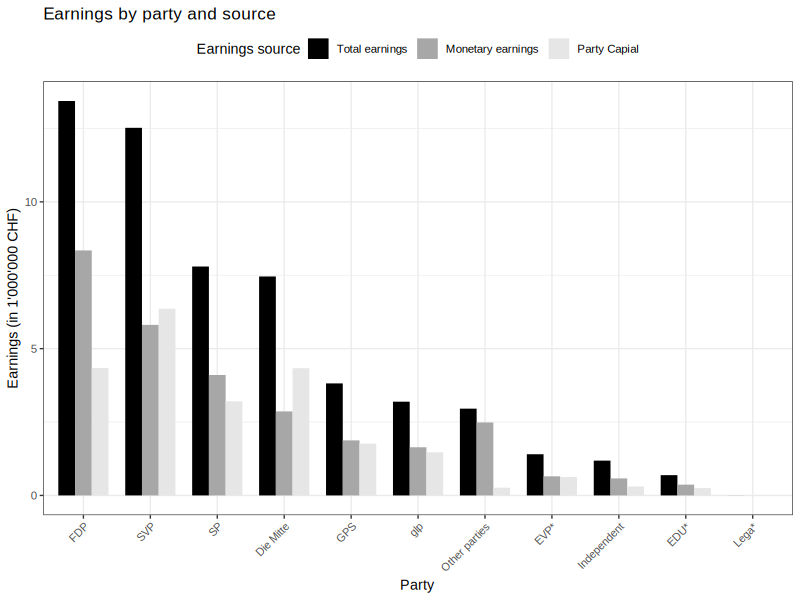
\includegraphics[width=1\linewidth]{output/plots/plot_figure_2.png}
    \caption{Earnings by party and source.}
    \floatfoot{\textit{Note: Non-monetary earnings, those through merchandise and events were ommitted for legibilty. Parties labelled * are not part of the analysis, as they were not able to form a faction in the large chamber of parliament after election day.}}
    \label{fig:fig2}
\end{figure}

\autoref{fig:fig3} depicts my operationalizations of party activity in the months leading up to the election: There seems to be ample variance between the parties in these metrics as well with the most active parties publishing three times as many posts on Instagram and issuing 8 times as many press releases as their least active counterparts. The bottom row puts the variables up to the parties’ budgets on the x-axis. This allows for a first assessment of the agency hypothesis H1: If it’s true that parties try to become more active influencers of the public agenda the higher their budgets are, then we should observe the lines in the bottom graphs to rise to the top-right, which is clearly not the case.
\begin{figure}
    \centering
    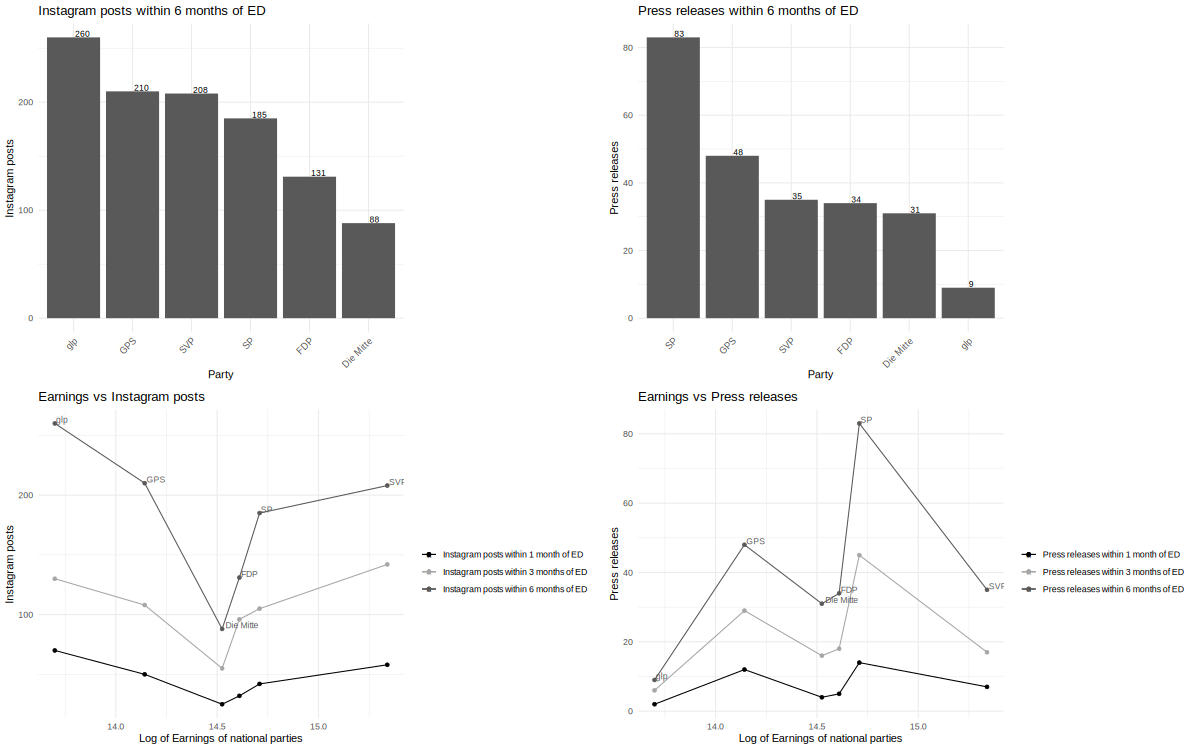
\includegraphics[width=1\linewidth]{output/plots/plot_figure_3.png}
    \caption{Party activity and earnings.}
    \floatfoot{\textit{Activity measured as the number of press releases (left) and posts on Instagram (right; top row) put against party earnings (bottom row). ED = Election Day.}}
    \label{fig:fig3}
\end{figure}
\autoref{fig:fig4} presents findings regarding the frequency hypothesis H2 in the same way: The bar plot shows the number of times a party appeared in the media within 6 months of the election, while the smooth conditional means graph plots them against the party’s campaign budget. Two significant observations can be drawn. Firstly, the two parties competing for the ecological vote (the GPS and the glp) seem to fight for media attention. While the glp is more relevant when considering the 6 months leading up to the election, the GPS is more salient within the last month. I want to argue that this is evidence in favor of H2: Because parties will be spending more money in the days and weeks leading up to the election than in the 6 months prior, the effect of a higher budget on the relevance in the media will be stronger the closer the election is. Thereby, the higher campaign budget of the GPS helped it become more relevant than the glp within the course of the election campaign. 
\begin{figure}
    \centering
    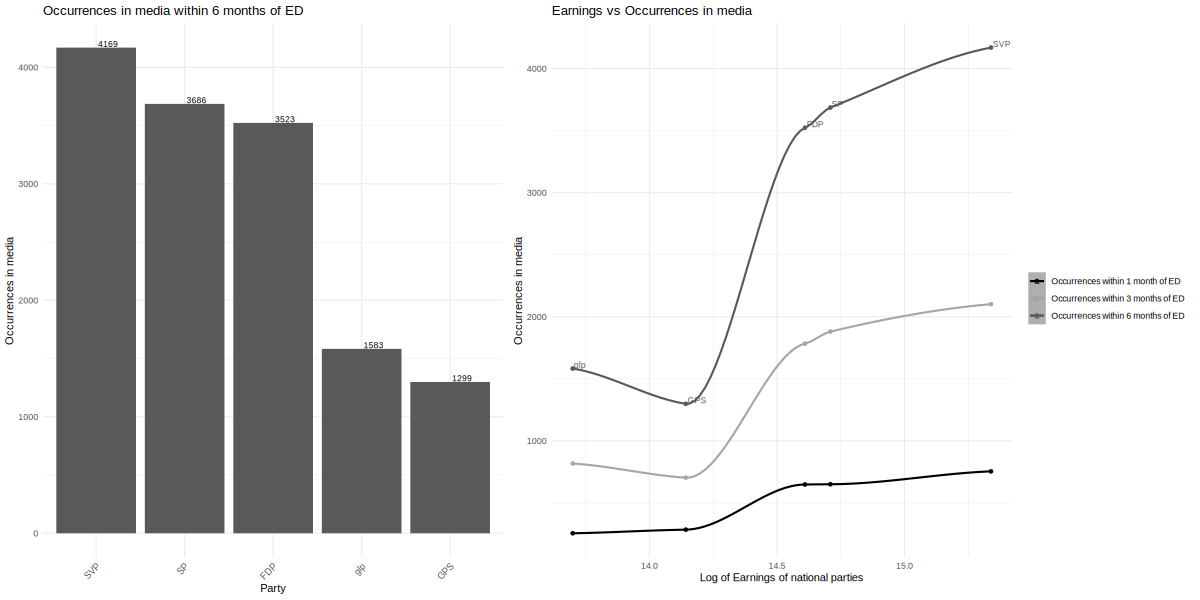
\includegraphics[width=1\linewidth]{output/plots/plot_figure_4.png}
    \caption{Occurrences and earnings.}
    \floatfoot{\textit{«Die Mitte» has been removed, See Appendix D for explanation. ED = Election day.}}
    \label{fig:fig4}
\end{figure}

Secondly, I want to take away that occurrences in the media are positively related to campaign budgets: Since the means line goes up over all – within the election month even without fail – I suggest the hypothesis withstands scrutiny with the selected data.

Next, I want to present descriptive statistics for the MISI scores in our dataset: \autoref{tab:tab3} displays the relevant summary statistics for MISI scores by CAP major topic. As becomes obvious from taking a look at the standard deviations, the variance of MISI score per topic is small: With a mean standard deviation of 0.006 MISI-points and an average mean-to-standard deviation ratio over 11.5:1, the spread of our index is tight. In other words: Within the data I chose, the media did not change its focus severely. A look at \autoref{fig:fig5} confirms this as well: Only a small number of trends can be identified, notably the continuous decline of \textit{«Domestic Commerce»}, the peak of \textit{«Environment»} three months ahead of the election, the rise of «Government Operations» towards the end of our dataset and the rapid uptick in reporting on \textit{«International Affairs»}. While the first two points are opaquer, an analysis of the articles in the latter two categories provides a clear explanation for their large rate of change: On October 7\textsuperscript{th} 2023, the terrorist organization Hamas attacked Israel, prompting Israel to respond with significant force, reinvigorating a long standing conflict. Against this backdrop, the use of the data I selected is problematic, as the issue salience hypothesis H3 which we try to test with it cannot incorporate such idiosyncrasies.


\begin{table}
\centering
\caption{Summary statistics for MISI distribution in the dataset by issue. }
\label{tab:tab3}
\vspace{0.5cm}
\begin{tabular*}{\linewidth}{@{\extracolsep{\fill}} | l | l | l | l | l | l |}
\hline
\textit{Issue Name} & \textit{Mean} & \textit{Median} & \textit{Std. Dev.} & \textit{Minimum} & \textit{Maximum} \\
\hline
\textbf{Agriculture} & 0.0175 & 0.0185 & 0.002 & 0.0153 & 0.0188 \\
\hline
\textbf{Civil Rights} & 0.0619 & 0.0618 & 0.0031 & 0.0589 & 0.0651 \\
\hline
\textbf{Culture} & 0.0539 & 0.0538 & 0.0029 & 0.0511 & 0.0569 \\
\hline
\textbf{Defense} & 0.052 & 0.0534 & 0.005 & 0.0464 & 0.0561 \\
\hline
\textbf{Dom. Comm.} & 0.167 & 0.166 & 0.0152 & 0.1522 & 0.1826 \\
\hline
\textbf{Education} & 0.0103 & 0.0095 & 0.0023 & 0.0085 & 0.0129 \\
\hline
\textbf{Energy} & 0.0171 & 0.0169 & 0.0006 & 0.0167 & 0.0177 \\
\hline
\textbf{Environment} & 0.0688 & 0.0655 & 0.0141 & 0.0568 & 0.0843 \\
\hline
\textbf{Foreign Trade} & 0.0082 & 0.0083 & 0.0002 & 0.008 & 0.0084 \\
\hline
\textbf{GovOps} & 0.0865 & 0.0923 & 0.0103 & 0.0747 & 0.0925 \\
\hline
\textbf{Health} & 0.0436 & 0.0439 & 0.0057 & 0.0377 & 0.0491 \\
\hline
\textbf{Housing} & 0.0134 & 0.0132 & 0.0012 & 0.0124 & 0.0148 \\
\hline
\textbf{Immigration} & 0.017 & 0.0162 & 0.0025 & 0.0151 & 0.0198 \\
\hline
\textbf{Intern. Affairs} & 0.127 & 0.1193 & 0.0356 & 0.0959 & 0.1659 \\
\hline
\textbf{Labor} & 0.0079 & 0.0067 & 0.0022 & 0.0065 & 0.0104 \\
\hline
\textbf{Law and Crime} & 0.1115 & 0.1122 & 0.0052 & 0.106 & 0.1163 \\
\hline
\textbf{Macroecon.} & 0.0171 & 0.0175 & 0.0023 & 0.0146 & 0.0191 \\
\hline
\textbf{Public Lands} & 0.0002 & 0.0002 & 0.0001 & 0.0001 & 0.0003 \\
\hline
\textbf{Social Welfare} & 0.0148 & 0.0149 & 0.0036 & 0.0111 & 0.0182 \\
\hline
\textbf{Technology} & 0.0364 & 0.0339 & 0.0057 & 0.0323 & 0.0429 \\
\hline
\textbf{Transport.} & 0.0678 & 0.0668 & 0.0063 & 0.0621 & 0.0745 \\
\hline

\end{tabular*}

\end{table}

\begin{figure}
    \centering
    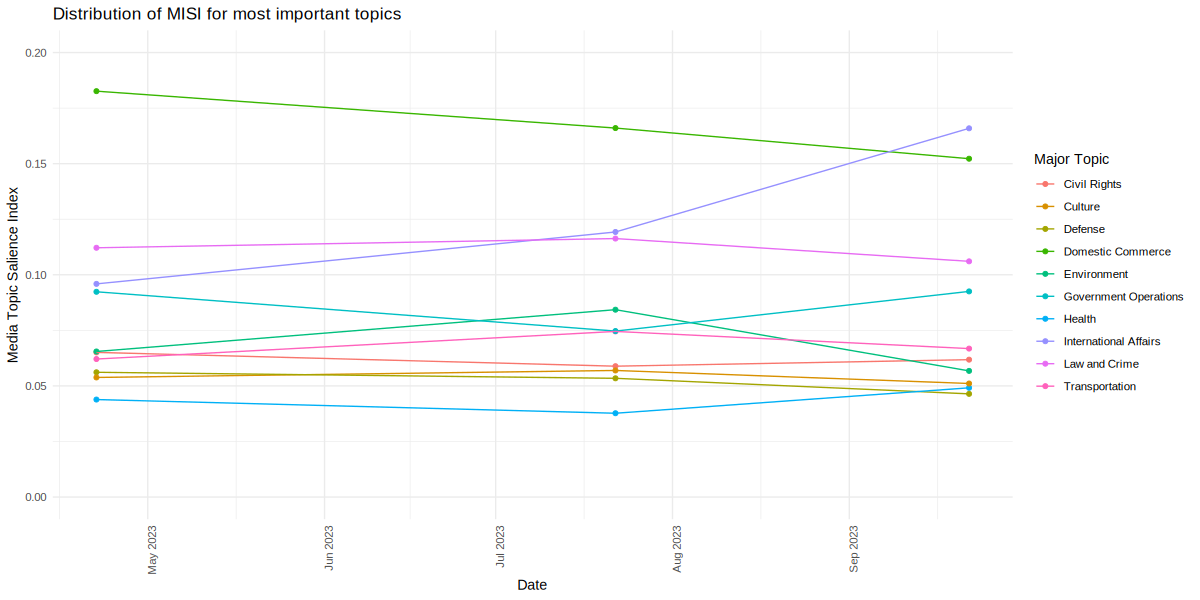
\includegraphics[width=1\linewidth]{output/plots/plot_figure_5.png}
    \caption{MISI distribution.}
    \floatfoot{\textit{10 Topics with the highest mean MISI.}}
    \label{fig:fig5}
\end{figure}

To describe the PISI data, I suggest picking the 5 most salient issues for each party: On the one hand, this allows for assertions surrounding issue-spread across parties. On the other, checking these topics against expectations of issue ownership (e.g. the intuition that SVP will focus on immigration or that the GPS will focus on environmental issues) will speak to the reliability of the index. \autoref{tab:tab4} displays these most important topics \textit{MIPs} and their respective PISI for each party.


\begin{table}
\centering
\caption{5 most important CAP topics listed by party with PISI scores in brackets.}
\label{tab:tab4}
\vspace{0.5cm}
\begin{tabular*}{\linewidth}{@{\extracolsep{\fill}} | l | l | l |}
\hline
\thead{SVP} & \thead{SP} & \thead{FDP} \\
\hline
    \footnotesize
    \makecell{1. Immigration (0.1338)\\
    2. International Affairs (0.0947)\\
    3. Civil Rights (0.0896)\\
    4. Energy (0.0788)\\
    5. Social Welfare (0.0714)}&     
    \footnotesize
    \makecell{1. Social Welfare (0.2313)\\
    2. International Affairs (0.1559)\\
    3. Civil Rights (0.1432)\\
    4. Macroeconomics (0.1398)\\
    5. Environment (0.0698)}&
    \footnotesize
    \makecell{1. Macroeconomics (0.2565)\\
    2. Social Welfare (0.1503)\\
    3. Energy (0.1402)\\
    4. Health (0.1069)\\
    5. Foreign Trade (0.1036)}\\
\hline
\thead{Die Mitte} & \thead{GPS} & \thead{glp} \\
\hline
    \footnotesize
    \makecell{1. Environment (0.1068)\\
    2. International Affairs (0.1054)\\
    3. Health (0.1008)\\
    4. Domestic Commerce (0.0880)\\
    5. Energy (0.0770)}&
    \footnotesize
    \makecell{1. Environment (0.1664)\\
    2. Civil Rights (0.1009)\\
    3. International Affairs (0.0960)\\
    4. Technology (0.0684)\\
    5. Energy (0.0600)}&
    \footnotesize
    \makecell{1. Environment (0.1565)\\
    2. Macroeconomics (0.0968)\\
    3. Health (0.0795)\\
    4. Transportation (0.0779)\\
    5. Civil Rights (0.0755)}\\
\hline

\end{tabular*}

\end{table}
From this list I am deducing that there is satisfactory variance in which topics parties are highlighting: More than half of the 21 CAP major topics are represented in the parties’ top 5 issues. Barring trends that are reflecting the political \textit{zeitgeist}, such as the fact that Die Mitte is talking about the environment most often, the results also confirm with appropriate assumptions: The SVP is, as expected, talking about immigration most often, the SP about Social Welfare, the FDP about Macroeconomics. Noteworthy are the differences in PISI-substantiveness as well: While the MIP-MISI scores for SP and FDP are rather large – the scores can be interpreted by saying that the SP and the FDP are talking about Social Welfare and Macroeconomics respectively one fourth of the time – these scores are smaller for Die Mitte and the SVP. This can be interpreted as certain parties not having as clear of a topical focus as others. While this might be reasonable for Die Mitte, such conclusions seem more unlikely when thinking about the SVP.


\subsection{Regression analysis}
\autoref{tab:tab5} includes the OLS coefficients for the 7 models I ran to test the issue salience hypothesis H3. I started with an empty model (1), pitting PISI against MISI\_1m, iteratively adding earnings, party controls, the interaction term and finally MISI\_3m and MISI\_6m, building up to the full model (7).



\begin{sidewaystable}
    \centering
    \resizebox{\textheight}{!}{%
    \begin{tabular}{@{\extracolsep{50pt}}lccccccc} 
    \\[-1.8ex]\hline 
    \hline \\[-1.8ex] 
     & \multicolumn{7}{c}{\textit{Dependent variable:}} \\ 
    \cline{2-8} 
    \\[-1.8ex] & \multicolumn{7}{c}{MISI within election month} \\ 
     & PISI & + log(Earnings) & + Controls & + Interaction & + MISI 3m & alt: MISI 6m & Full Model \\ 
    \\[-1.8ex] & (1) & (2) & (3) & (4) & (5) & (6) & (7)\\ 
    \hline \\[-1.8ex] 
     PISI & 0.095$^{+}$ & 0.095$^{+}$ & 0.095$^{+}$ & 4.986$^{*}$ & $-$0.709$^{+}$ & 0.782$^{+}$ & $-$0.907$^{+}$ \\ 
      & (0.086) & (0.087) & (0.088) & (2.808) & (0.860) & (1.082) & (0.875) \\ 
      & & & & & & & \\ 
     Log of Party Earnings &  & $-$0.000 & $-$0.000 & 0.015$^{+}$ & $-$0.002$^{+}$ & 0.002 & $-$0.003$^{+}$ \\ 
      &  & (0.008) & (0.013) & (0.015) & (0.005) & (0.006) & (0.005) \\ 
      & & & & & & & \\ 
     Number of Seats &  &  & 0.000 & 0.000 & 0.000 & 0.000 & 0.000 \\ 
      &  &  & (0.001) & (0.001) & (0.0002) & (0.0003) & (0.0002) \\ 
      & & & & & & & \\ 
     Left-Right Scale &  &  & 0.000 & 0.000 & 0.000 & 0.000 & 0.000 \\ 
      &  &  & (0.004) & (0.003) & (0.001) & (0.001) & (0.001) \\ 
      & & & & & & & \\ 
     GAL-TAN Scale &  &  & $-$0.000 & $-$0.000 & 0.000 & 0.000 & 0.000 \\ 
      &  &  & (0.004) & (0.004) & (0.001) & (0.001) & (0.001) \\ 
      & & & & & & & \\ 
     MISI 3 months before ED &  &  &  &  & 1.010$^{***}$ &  & 1.169$^{***}$ \\ 
      &  &  &  &  & (0.029) &  & (0.137) \\ 
      & & & & & & & \\ 
     MISI 6 bonths before ED &  &  &  &  &  & 0.967$^{***}$ & $-$0.161$^{+}$ \\ 
      &  &  &  &  &  & (0.037) & (0.135) \\ 
      & & & & & & & \\ 
     PISI * Log of Party Earnings &  &  &  & $-$0.307$^{*}$ & 0.046$^{+}$ & $-$0.046$^{+}$ & 0.058$^{+}$ \\ 
      &  &  &  & (0.176) & (0.054) & (0.068) & (0.055) \\ 
      & & & & & & & \\ 
     Constant & 0.043$^{***}$ & 0.043 & 0.043 & $-$0.190$^{+}$ & 0.033$^{+}$ & $-$0.036$^{+}$ & 0.043$^{+}$ \\ 
      & (0.006) & (0.120) & (0.189) & (0.230) & (0.069) & (0.088) & (0.070) \\ 
      & & & & & & & \\ 
    \hline \\[-1.8ex] 
    Observations & 126 & 126 & 126 & 126 & 126 & 126 & 126 \\ 
    R$^{2}$ & 0.010 & 0.010 & 0.010 & 0.034 & 0.913 & 0.861 & 0.914 \\ 
    Adjusted R$^{2}$ & 0.002 & $-$0.006 & $-$0.032 & $-$0.014 & 0.908 & 0.853 & 0.909 \\ 
    Residual Std. Error & 0.046 (df = 124) & 0.046 (df = 123) & 0.047 (df = 120) & 0.046 (df = 119) & 0.014 (df = 118) & 0.018 (df = 118) & 0.014 (df = 117) \\ 
    F Statistic & 1.204$^{+}$ (df = 1; 124) & 0.597$^{+}$ (df = 2; 123) & 0.233 (df = 5; 120) & 0.704$^{+}$ (df = 6; 119) & 177.846$^{***}$ (df = 7; 118) & 104.421$^{***}$ (df = 7; 118) & 156.337$^{***}$ (df = 8; 117) \\ 
    \hline 
    \hline \\[-1.8ex] 
    \textit{Note:}  & \multicolumn{7}{r}{$^{+}$p$<$0.1; $^{*}$p$<$0.1; $^{**}$p$<$0.05; $^{***}$p$<$0.01} \\ 
    \end{tabular} 
    }
    \caption{Table representing regression model coefficients.}
    \label{tab:tab5}
\end{sidewaystable}


I want to draw attention to 5 findings: Firstly, the coefficients for PISI, Party earnings and the interaction term do not achieve a p-value lower than 0.1 in most models. This supports the finding that, in our data, no significant correlation between these three covariates and MISI\_1m can be established.

Secondly, I want to draw attention to the significant and substantial correlation between the MISI controls and the MISI dependent variable: In both model (5) and (6) MISI\_3m and MISI\_6m correlated with MISI\_1m nearly perfectly. This supports the finding from above that the media issue salience did not change pronouncedly in the 6 months leading up to the election.

The third point I want to make is that I ran regressions with a limited number of observations. Because my level of observation was the party-topic dyad and I analyzed 21 topics for 6 parties, this leaves us with 126 observations. I’d argue that if there was more data available or a different level of analysis had been used, the coefficients would allow for more comprehensive detections.

As a fourth finding, I want to point out the one occurrence of a PISI p-value lower than 0.1: When adding the term measuring the interaction between PISI and earnings in model (4), the coefficient for PISI achieves a statistically significant confidence and its predictive power grows substantially compared to model (3). I’d argue this supports the conclusion, that when holding the interaction between party issue salience and the party’s resources constant, their issue salience influences the media agenda, as opposed to when letting the interaction vary where it does not. While this finding does not support H3 specifically, it does hint to some connection between party earnings and party issue salience. Nonetheless, allow me to add some limitations: The R\textsuperscript{2} of all models not containing MISI controls are minimal. Even though the indicator grows by a factor of four when moving from model (3) to model (4), it still only reaches a value of 0.04, meaning only 4\% of the variance in the dataset can be explained through this model. Additionally, the F-tests fail: Though it could be argued that this should lead to the immediate dismissal of all models that do not contain MISI controls – as they are the only ones with significant F-Stats – I want to suggest that the increase in substantially and the decrease of the p-value when moving from (3) to (4) and thereby the implied connection between earnings and salience stand independently of the F-test. Furthermore, the low number of cases and covariates do not put the regression models at risk of coincidental correlation through regression towards the mean.

As my fifth and final insight, I want to highlight that when lowering the confidence cutoff to 70\%, the PISI coefficient is significant even when controlling for the MISI index 6 months prior as shown in model (6). As I have made a succinct case that the underlying data is flawed, I posit that lowering the threshold in this case is suitable.\footnote{Regression table including p-values available in the code repository in «output/tables/table\_5\_with\_pvalues.html».}


\section{Conclusions, caveats, and contributions}
Let me preface the final chapter of my thesis by summarizing my findings in regards to the three hypotheses I proposed: I was not able to provide evidence for the agency hypothesis H1 based on my data. Descriptive evidence substantiated the frequency hypothesis H2 and the regression models I ran supplied inconclusive evidence for the issue salience hypothesis H3. I will finalize this thesis by listing conclusions, caveats and scientific contributions I argue this paper has made, climaxing in a few final thoughts discussing this paper's consequences.


\subsection{Conclusions: What did we learn?}
\begin{enumerate}
    \item \textit{What if we just measured MISI and PISI wrongly?} The fourth and fifth finding in my regression analysis leads me to argue that the inferred connection between PISI and MISI could not be made, because the data does not accurately measure the underlying concepts or it is flawed through factors out of my control. I want to use this discovery, not to make the case that H3 can be substantiated through my analysis but to stipulate that there is reason to keep investigating.
    \item \textit{What if elite-constructionism does not work this quickly?} The finding that media salience is very robust seems to suggest that the media «does not change its mind through elite-influence». I would append this statement by a temporal component: Had we used data for a longer time frame, the stability of the media agenda might decrease. Enlarging this horizon would allow us to make clearer conclusions on the whodunnit of media-elite-relationships. Additionally, qualitative research in the form of mechanism tracing and extensive case studies would allow for further enhancement of the framework of this thesis. As a fitting case in the confines of this study, I want to suggest analyzing the appearance of the \textit{«10 Millionen Schweiz»}-Frame which was propagated by the SVP and promptly dropped come election day. 
\end{enumerate}


\subsection{Caveats: Could we learn more?}
\begin{enumerate}
    \item \textit{What if we used different and more PISI source material?} Although the descriptive analysis of the PISI scores per party revealed that the index I created matched the expectations connoisseurs of the Swiss political landscape are likely to have, the way in which I calculated it comes with some unavoidable drawbacks: Election platforms and comprehensive party programs in particular are inherently rigid, as they are most often authorized by general assemblies or party conventions. While they serve as guidance for a party’s communication in general, they can never be complete. Adding the content of more publications, such as blog posts, newsletters or press releases, or even switching the domain to code parliamentary speaches would definitely improve the validity, reliability and generalizability of the index. Doing so could help answering open questions such as the fact that the SVP’s counterintuitively talks very little about immigration compared to the issue salience of Macroeconomics for the FDP. Furthermore, coding publictions throughout the election period, such as articles or press releases created in the election campaign, might resolve the problem about PISI responsiveness: If we include data measuring how parties react to (keyword: culturalist-constructivism) or shape (keyword: elite-constructivism) the media agenda on political happenings such as the Israeli-Palestinian war in our PISI measurment, I want to claim that broader conclusions could be made.

    \item  \textit{Is there a different way of testing H1 and H2?} Because of the way I operationalized party activity and relevance in the media, I was not able to run regressions to test these two hypotheses. There are two ways in which this problem could be resolved: Either, we add more data by expanding the levels of analysis to the cantonal level, operationalizing the regressand differently or by waiting for more data to become available. As the budget declaration obligation by the audit office also applies to direct democratic votes and Switzerland holds several votes per year, it is only a matter of time until such calculations can be done through statistical means. Alternatively, qualitative case studies could analyze the behaviour of campaigning parties, inductively enhancing the framework of how money shapes the agenda setting process.

    \item \textit{Are earnings and spending levels congruent?} The dataset on campaign finances includes levels of campaign earnings, not of \textit{spendings}. Judging whether these two measures are congruent is impossible with the methods I have chosen and is therefore assumed. Further research should address possible ways in which this conundrum could be resolved or, alternatively, spendings data should have to be reported and made available for scientific research by changing the regulation.

    \item \textit{Was it the right time to conduct this analysis?} It would be pretentious not to address the fact that I analyzed issue salience in the media when, because of a human catastrophy, the salience of international affairs rose substantially. And yet, there seemingly is no way to control for this anomaly through skew correction or other statistical methods. Replication of this analysis in a media environment where no stories about terror and war are on the frontpages is advisable. 



\end{enumerate}

\subsection{Contributions: How did this paper help us learn?}
\begin{enumerate}
    \item  \textit{A fair, novel framework and operationalizations:} By providing a summary of a large body of literature and logically deriving two premises, I was able to build a parsimonious framework that I argue to be a fair and original lense through which to appreciate the connection of money and politics. I posit this to be the most far-reaching contribution my paper makes as the ways in which this model can be applied and the hypotheses to be derived from it are numerous. The operationalization of issue salience for parties and media – the PISI and MISI scores – seem equally useful.

    \item \textit{Machine readability and CAP Coding of Swiss party positions:} As far as I am able to tell, party programs of Swiss parties have not been coded into CAP topics so far. The data made available in the code repository in Appendix B – including the plaintext versions of the newest party program by SVP, the election platforms by FDP, GPS and SP that are not yet available in the Manifesto Project Database and the PISI data – may be used for scientific research indiscrimintely. 

    \item \textit{Argument to fine-tune CAP topics:} As the creator of the CAP master codebook Shaun Bevan (\citeyear{bevan_gone_2019}) denotes himself, the CAP Major topic categorization has several limitations. A look at the different content-widths (compare «Macroeconomics», a relatively wide topic, and «Public Lands», a very narrow topic) and content-typologies (compare «Social Welfare», an ideological distinction, and «Government Operations», a legal distinction) suffices to conclude that a harmonization of topics is called for. This paper adds to the heap of literature that advocates for such an overhaul. Think about Die Mitte’s topics: Formerly Supporting the nuclear family, which is one of the core topics of their ideology, would fall into «Law and Crime». The appropriateness of this classification is in my opinion questionable. 

    \item \textit{Application of an AI method}: Through the use of an AI-assisted content analysis solution and the discussion of its validity, I have provided further evidence for the specific method’s validity and the usefulness of machine learning methods in the social sciences.

\end{enumerate}

\subsection{Final remarks: What of it?}
It is now time to ask: \textit{What are the consequences of the findings this paper has made?} I must highlight once more that I was not able to find any evidence for my third and most far-reaching \textit{issue salience hypothesis} to a reasonable degree of scientific certainty. And yet, I want to argue that it would be negligent to infer no connection between financial resources, party issue salience and the media's agenda and therefore financial resources do not influence electoral outcomes through the mechanism I proposed: We must not throw the baby out with the bath water! Even the most doubtful readers, the ones most skeptical of accusations of oligarchical foul play by the high society and wealthy corporations, can't overlook the PISI jump in significance from model (3) to model (4) and its significance, even when controlling for media issue salience merely 180 days prior. While the data clearly does not allow for any sweeping prophecies, there's no denying it: This paper can serve as the foundation for future analysis into the influence of money in politics.


\newpage

\printbibliography
\addcontentsline{toc}{section}{\protect\numberline{}References}

\newpage
\pagenumbering{gobble}
\vspace*{\fill}
\begin{center}
    \Large\textbf{Disclaimer on the use of artificial intelligence:}\\
    \normalsize
    \textit{
        The contents of the following paper were written entirely without the use of artificially intelligent text generation models. The literature cited was found in part with the use of two AI-powered tools, namely researchrabbit.ai and scite.ai. While the exact use of researchrabbit.ai is practically impossible to reconstruct, the author believes the simple disclosure of its use will class under the fair-disclosure of AI-tools and will therefore be allowed under the statement of authorship provided by the University of Zurich. The prompts used with scite.ai can be found in Appendix E of this document. No further AI-implements, including but not limited to ChatGPT, Bard, Copilot or Bing Chat, were used.
    }
\end{center}
\vspace*{\fill}

\newpage
\pagenumbering{Roman}
\section*{Appendix}
\addcontentsline{toc}{section}{\protect\numberline{}Appendix}

\subsection*{\textsc{Appendix A}: Query configuration to the SMD through Swissdox@LiRI}
\addcontentsline{toc}{subsection}{\protect\numberline{}\textsc{Appendix A}: Query configuration to the SMD through Swissdox@LiRI}

\underline{For H2}

\begin{multicols}{2}

\footnotesize
\begin{verbatim}
    Query «SVP»
    query:
      sources:
        - ZWA
        - ZWAO
        - TA
        - NNTA
        - NZZO
        - NZZ
        - NZZS
        - TAS
        - SRF
      dates:
        - from: 2023-04-22
          to: 2023-10-21
      languages:
        - de
      doctypes:
        - WWE
        - PND
        - PLD
        - PID
        - PRD
        - PJO
        - NNE
      content:
        - Schweizerische Volkspartei
        - schweizerische Volkspartei
        - SVP
    result:
      format: TSV
      maxResults: 10000000
      columns:
        - id
        - pubtime
        - medium_code
        - medium_name
        - rubric
        - regional
        - doctype
        - doctype_description
        - language
        - char_count
        - dateline
        - head
        - subhead
        - content_id
        - content
    version: 1.2
\end{verbatim}

\newpage
\begin{verbatim}
    Query «SP»
    query:
      sources:
        - ZWA
        - ZWAO
        - TA
        - NNTA
        - NZZO
        - NZZ
        - NZZS
        - TAS
        - SRF
      dates:
        - from: 2023-04-22
          to: 2023-10-21
      languages:
        - de
      doctypes:
        - WWE
        - PND
        - PLD
        - PID
        - PRD
        - PJO
        - NNE
      content:
        - Sozialdemokratische Partei
        - sozialdemokratische Partei
        - SP
    result:
      format: TSV
      maxResults: 10000000
      columns:
        - id
        - pubtime
        - medium_code
        - medium_name
        - rubric
        - regional
        - doctype
        - doctype_description
        - language
        - char_count
        - dateline
        - head
        - subhead
        - content_id
        - content
    version: 1.2

\end{verbatim}

\newpage

\begin{verbatim}
    Query «FDP»
    query:
      sources:
        - ZWA
        - ZWAO
        - TA
        - NNTA
        - NZZO
        - NZZ
        - NZZS
        - TAS
        - SRF
      dates:
        - from: 2023-04-22
          to: 2023-10-21
      languages:
        - de
      doctypes:
        - WWE
        - PND
        - PLD
        - PID
        - PRD
        - PJO
        - NNE
      content:
        - FDP
        - FDP.Die Liberalen
        - fdp
    result:
      format: TSV
      maxResults: 10000000
      columns:
        - id
        - pubtime
        - medium_code
        - medium_name
        - rubric
        - regional
        - doctype
        - doctype_description
        - language
        - char_count
        - dateline
        - head
        - subhead
        - content_id
        - content
    version: 1.2
\end{verbatim}

\newpage

\begin{verbatim}
    Query «GRÜNE»
    query:
      sources:
        - ZWA
        - ZWAO
        - TA
        - NNTA
        - NZZO
        - NZZ
        - NZZS
        - TAS
        - SRF
      dates:
        - from: 2023-04-22
          to: 2023-10-21
      languages:
        - de
      doctypes:
        - WWE
        - PND
        - PLD
        - PID
        - PRD
        - PJO
        - NNE
      content:
        - GRÜNE
        - die Grüne
        - Die Grünen
        - die Grünen
        - grüne Partei
    result:
      format: TSV
      maxResults: 10000000
      columns:
        - id
        - pubtime
        - medium_code
        - medium_name
        - rubric
        - regional
        - doctype
        - doctype_description
        - language
        - char_count
        - dateline
        - head
        - subhead
        - content_id
        - content
    version: 1.2
\end{verbatim}

\newpage

\begin{verbatim}
    Query «glp»
    query:
      sources:
        - ZWA
        - ZWAO
        - TA
        - NNTA
        - NZZO
        - NZZ
        - NZZS
        - TAS
        - SRF
      dates:
        - from: 2023-04-22
          to: 2023-10-21
      languages:
        - de
      doctypes:
        - WWE
        - PND
        - PLD
        - PID
        - PRD
        - PJO
        - NNE
      content:
        - glp
        - GLP
        - grünliberale Partei
        - Grünliberale
        - Grünliberalen
    result:
      format: TSV
      maxResults: 10000000
      columns:
        - id
        - pubtime
        - medium_code
        - medium_name
        - rubric
        - regional
        - doctype
        - doctype_description
        - language
        - char_count
        - dateline
        - head
        - subhead
        - content_id
        - content
    version: 1.2
\end{verbatim}

\newpage

\underline{For H3}

\begin{verbatim}
    Query «month 1 before ED»
    query:
      sources:
        - ZWA
        - ZWAO
        - TA
        - NNTA
        - NZZ
        - NZZO
        - NZZS
        - TAS
        - SRF
      dates:
        - from: 2023-09-22
          to: 2023-10-21
      languages:
        - de
      doctypes:
        - PID
        - PLD
        - PND
        - NNE
        - WWE
        - PRD
        - PJO
        - PLW
        - PMA
    result:
      format: TSV
      maxResults: 10000000
      columns:
        - id
        - pubtime
        - medium_code
        - medium_name
        - rubric
        - regional
        - doctype
        - doctype_description
        - language
        - char_count
        - dateline
        - head
        - subhead
        - content_id
        - content
    version: 1.2
\end{verbatim}

\newpage

\begin{verbatim}
    Query «month 3 before ED»
    query:
      sources:
        - ZWA
        - ZWAO
        - TA
        - NNTA
        - NZZ
        - NZZO
        - NZZS
        - TAS
        - SRF
      dates:
        - from: 2023-07-22
          to: 2023-08-21
      languages:
        - de
      doctypes:
        - PID
        - PLD
        - PND
        - NNE
        - WWE
        - PRD
        - PJO
        - PLW
        - PMA
    result:
      format: TSV
      maxResults: 10000000
      columns:
        - id
        - pubtime
        - medium_code
        - medium_name
        - rubric
        - regional
        - doctype
        - doctype_description
        - language
        - char_count
        - dateline
        - head
        - subhead
        - content_id
        - content
    version: 1.2
\end{verbatim}

\newpage

\begin{verbatim}
    Query «month 6 before ED»
    query:
      sources:
        - ZWA
        - ZWAO
        - TA
        - NNTA
        - NZZ
        - NZZO
        - NZZS
        - TAS
        - SRF
      dates:
        - from: 2023-04-22
          to: 2023-05-21
      languages:
        - de
      doctypes:
        - PID
        - PLD
        - PND
        - NNE
        - WWE
        - PRD
        - PJO
        - PLW
        - PMA
    result:
      format: TSV
      maxResults: 10000000
      columns:
        - id
        - pubtime
        - medium_code
        - medium_name
        - rubric
        - regional
        - doctype
        - doctype_description
        - language
        - char_count
        - dateline
        - head
        - subhead
        - content_id
        - content
    version: 1.2
\end{verbatim}

\end{multicols}

\normalsize

\newpage

\subsection*{\textsc{Appendix B}: Statement on code and data availability}
\addcontentsline{toc}{subsection}{\protect\numberline{}\textsc{Appendix B}: Statement on code and data availability}
All code used for the analysis and the data I am able to share in accordance with LiRI’s \textit{Terms of Use} etc. is available here: \href{https://github.com/stud-ipz-uzh/timothyjustinoesch_ba}{https://github.com/stud-ipz-uzh/timothyjustinoesch\_ba}. LiRI data can be accessed through the use of the queries provided above. Should the need arise, please contact me for support.


\newpage
\subsection*{\textsc{Appendix C}: Party publications used for H3 }
\addcontentsline{toc}{subsection}{\protect\numberline{}\textsc{Appendix C}: Party publications used for H3}

\begin{enumerate}
    \item SVP
    \begin{itemize}
        \item Name: «Parteiprogramm 2023 – 2027»
        \item Type: Party Program.
        \item Word count: 17’063 words
        \item Source: \href{https://www.svp.ch/wp-content/uploads/230726_Parteiprogramm.pdf}{https://www.svp.ch/wp-content/uploads/230726\_Parteiprogramm.pdf}
        \item Last accessed: 25.04.2024.
        \item Adopted on: 28.01.2023.
        \item Authorized by: General Assembly.
        \item Specific modifications: Removal of chapter recaps because of distortion concerns.
    \end{itemize}
\item SP
    \begin{itemize}
        \item Name: «WAHLEN 2023: WIR ERGREIFEN PARTEI.»
        \item Type: Election platform.
        \item Word count: 2’501 words.
        \item Source: \href{https://www.sp-ps.ch/wp-content/uploads/2022/10/Wahlplattform_Broschure_A5_D.pdf}{https://www.sp-ps.ch/wp-content/uploads/2022/10/Wahlplattform\_Broschure\_A5\_D.pdf}
        \item Last accessed: 25.04.2024.
        \item Adopted on: 29.10.2022.
        \item Authorized by: General Assembly.
        \item Specific modifications: None.
    \end{itemize}

\newpage
\item FDP
    \begin{itemize}
        \item Name: «Wir machen die Schweiz stark! Wahlkampfprogramm der FDP.Die Liberalen»
        \item Type: Election platform.
        \item Word count: 1'141 words.
        \item Source: \url{https://www.fdp.ch/fileadmin/documents/fdp.ch/pdf/DE/Dokumente/20230506_Wahlkampfprogramm_d.pdf}
        \item Last accessed: 25.04.2024.
        \item Adopted on: Unclear.
        \item Authorized by: Unclear.
        \item Specific modifications: Adding of «Wir fordern: » to bullet-point style demands if necessary for clearer coding.
    \end{itemize}

\item Die Mitte
    \begin{itemize}
        \item Name: Inapplicable
        \item Type: Positions from their webpage.
        \item Word count: 2’977 words.
        \item Source: \url{https://die-mitte.ch/themen}
        \item Last accessed: 25.04.2024.
        \item Adopted on: Unclear.
        \item Authorized by: Unclear.
        \item Specific modifications: Adding of «Wir fordern: » to bullet-point style demands if necessary for clearer coding.
    \end{itemize}

\newpage
\item GPS
    \begin{itemize}
        \item Name: «AGENDA 2023-2027 GRÜNES WAHLPROGRAMM»
        \item Type: Election platform.
        \item Word count: 16’610 words.
        \item Source: \url{https://gruene.ch/wp-content/uploads/2022/11/Agenda2023_Version_2_d_final.pdf}
        \item Last accessed: 25.04.2024.
        \item Adopted on: 28.01.2023.
        \item Authorized by: General Assembly.
        \item Specific modifications: Adding of «Wir fordern: » to bullet-point style demands if necessary for clearer coding.
    \end{itemize}

\item glp
    \begin{itemize}
        \item Name: «Leitlinien»
        \item Type: Party program.
        \item Word count: 3’431 words.
        \item Source: \url{https://grunliberale.ch/dam/jcr:7dac72fc-ec06-4d0f-bbee-f779a00cd265/Leitlinien_glp_D.pdf}
        \item Last accessed: 25.04.2024.
        \item Adopted on: 11.10.2014.
        \item Authorized by: General assembly.
        \item Specific modifications: None.
    \end{itemize}
\end{enumerate}

\newpage
\subsection*{\textsc{Appendix D}: Explanation for removing \textit{«Die Mitte»} from analysis of H2.}
\addcontentsline{toc}{subsection}{\protect\numberline{}\textsc{Appendix D}: Explanation for removing \textit{«Die Mitte»} from analysis of H2.}
As «die Mitte» simply translates to «the center» from German, there was no way to identify the party in the news articles database. Simply filtering for the party’s name, which returned satisfactory results for the other parties, understandably resulted in oversampling. Therefore, «die Mitte» was removed from analysis of H2. Future research will have to be conducted in order to resolve this issue.

\newpage
\subsection*{\textsc{Appendix E}: Prompts used with \textit{scite.ai}}
\addcontentsline{toc}{subsection}{\protect\numberline{}\textsc{Appendix E}: Prompts used with \textit{scite.ai}}
\setlength\parindent{0pt}

The following are prompts used with scite.ai. The prompts are in \textbf{bold}, the responses are \textit{italicized}. Prompt-typos were not removed.

\textbf{Find papers in the field of political science that argue different positions on the question wether the mass media influence the political agenda or political elites influence the agenda of the mass media.}

\textit{The influence of mass media on the political agenda and the reciprocal influence of political elites on media agenda-setting have been subjects of extensive research in political science. (2010) argue that the capacity of mass media to influence political parties' agendas is contingent upon the interests of the parties, suggesting a conditional relationship between mass media attention and political party agendas (Green-Pedersen \& Stubager, 2010). On the other hand, Wirth et al. (2010) found that the agenda of issues presented by political elites, such as presidents, influenced the subsequent national press agenda, indicating the influence of political elites on media agenda-building (Wirth et al., 2010). Additionally, Walgrave et al. (2007) and Walgrave \& Aelst (2006) have contributed to the understanding of the mass media's role in determining the political agenda, emphasizing the contingency and preliminary theory of media's political agenda-setting power (Walgrave et al., 2007; Walgrave \& Aelst, 2006). Furthermore, Vesa et al. (2015) revisited the politicians' views on the media's political agenda-setting power, highlighting the different perspectives on the extent of media influence on the political agenda (Vesa et al., 2015).}

 \textit{These studies collectively demonstrate the complex and multifaceted nature of the relationship between mass media and political elites in shaping the political agenda. While some research emphasizes the conditional nature of media influence on political parties, others highlight the significant influence of political elites on media agenda-setting. The synthesis of these references underscores the need for a nuanced understanding of the interplay between mass media and political elites in shaping the political agenda.}
\\
\\
 \textbf{Can you find more papers that argue the point that political elites, especially campaigns and campaigners, influence the mass media?}

\textit{The influence of political elites, particularly campaigns and campaigners, on the mass media has been a subject of scholarly inquiry (Thesen, 2013). highlights the importance of investigating the media's role in promoting social problems on the political agenda, emphasizing the mediatized politics perspective (Thesen, 2013). Additionally, Aelst \& Walgrave (2017) propose an actor-centered, functional approach to understanding the dual function of the news media for political elites, shedding light on the influence of political actors on media agenda-setting (Aelst \& Walgrave, 2017). Furthermore, Davis (2003) points out documented cases of elites being influenced in their decision-making by media campaigns, underscoring the reciprocal relationship between political elites and the mass media (Davis, 2003). Moreover, (2012) discusses negotiation between elites outside the public sphere of mass media, indicating the significant influence of political elites in shaping agendas (Örnebring, 2012). These references collectively contribute to the understanding of the influence of political elites, especially campaigns and campaigners, on the mass media, highlighting the complex interplay between political actors and media agenda-setting.}
\\
\\
 \textbf{Find papers in the field of political science that analyse the connection between campaign spending and the media agenda.}

\textit{The relationship between campaign spending and the media agenda has been a subject of interest in political science research. Studies have shown that the media plays a significant role in shaping the political agenda during election campaigns (Walgrave \& Aelst, 2006). The influence of the media on campaign agendas has been a focus of research, with some studies indicating that parties set the agenda of the media during elections (Vliegenthart \& Walgrave, 2010). Additionally, the intermedia agenda-setting relationships between news media coverage and political ads generated by campaigns have been highlighted as an area requiring further investigation (Ragas \& Kiousis, 2010). Furthermore, the impact of social media on agenda building during election campaigns has been examined, with research indicating that Twitter communication by parties and politicians shapes the media agenda (Seethaler \& Melischek, 2019). It has also been suggested that mass media can set the public’s agenda, particularly during political campaigns (Towner \& Munoz, 2020).}

 \textit{The influence of the media on campaign agendas has been studied through various theoretical perspectives, including agenda-setting theory (Seethaler \& Melischek, 2019). Research has also compared the contributions of political news releases and advertisements on media content during political campaigns, highlighting their relative linkages with news content (Kiousis et al., 2009). Furthermore, the flow of arguments among campaigners, the media, and the public in shaping the agenda during referendum campaigns has been investigated (Wirth et al., 2010). The role of issue content in campaign advertising and its interaction with the interests and agendas of issue publics has also been examined (Sides \& Karch, 2008).}

 \textit{In addition to traditional media, the impact of social media platforms such as Twitter on agenda building during election campaigns has been a subject of interest (Sarma \& Hazarika, 2023). The usage of social media by political parties to influence the public agenda has been highlighted, with a focus on the spread of negative campaigns about opposition parties and the promotion of their own agendas (Sarma \& Hazarika, 2023).}

 \textit{Overall, the literature suggests that the relationship between campaign spending and the media agenda is complex and multifaceted, involving traditional media, social media, political parties, and issue content. Further research is needed to fully understand the dynamics of this relationship and its implications for political communication and public opinion formation during election campaigns.}
\\
\\
 \textbf{Find papers in the field of political science that highlight the controversy wether campaign funds matter for electoral success or not.}

\textit{The impact of campaign funds on electoral success has been extensively researched in political science. Studies have examined the relationship between campaign spending and electoral outcomes, with some finding that higher campaign spending is associated with increased electoral success (Jucá et al., 2016). However, there are debates on whether restricting campaign spending would lead to electoral parity (Fisher et al., 2013). Additionally, research suggests that media coverage of campaign events significantly affects candidates' chances for electoral success (Shaw \& Roberts, 2000; Erkel et al., 2018).}

 \textit{The role of public funding in influencing electoral competitiveness and candidate success has also been explored. Advocates of public funding argue that it reduces corruption and increases electoral competitiveness, while critics argue that it imposes unjust burdens on candidates (Werner \& Mayer, 2007; Ortuño-Ortín \& Schultz, 2005). Furthermore, philanthropic practices have been shown to contribute to electoral success (A'isyah \& Lessy, 2022).}

 \textit{In conclusion, the literature presents a complex and multifaceted debate on the relationship between campaign funds and electoral success, with studies offering conflicting perspectives on the impact of campaign spending, media attention, and public funding.}
\\
\\
 \textbf{Find papers that support the conclusion that campaign finance does not matter for the outcome of elections}

\textit{The literature presents a diverse range of perspectives on the impact of campaign finance on electoral outcomes. Bean challenges the notion of the rational voter and suggests that democracies may choose bad policies, implying that campaign finance may not significantly influence electoral outcomes . Stratmann provides a partial review of the literature on money in politics, indicating that the relationship between campaign finance and electoral success is not straightforward . Furthermore, Bjornlund presents evidence supporting the idea that public campaign financing affects judicial legitimacy, suggesting that campaign finance may have limited impact on electoral outcomes . Porter and Steelman investigate the success of political newcomers in elections and highlight the role of early donations, indicating that factors beyond campaign finance may influence electoral success . Additionally, Butcher and Milyo examine the impact of campaign finance reforms on incumbent competition, suggesting that such reforms may not insulate incumbents from competition . Gross and Goidel explore the impact of state campaign finance laws and their findings suggest that these laws may not have a systematic influence on electoral outcomes .}

 \textit{These studies collectively provide a nuanced understanding of the relationship between campaign finance and electoral success, indicating that the impact of campaign finance on electoral outcomes is complex and multifaceted.}
\\
\\
 \textbf{Find papers in the field of political science that analyse how the public agenda influences the outcome of elections.}

\textit{To understand how the public agenda influences the outcome of elections, it is essential to consider the interplay between public opinion, media influence, and policy responsiveness (Stimson, 1995). highlights that elections can change the government's political composition, leading to new policies, while policymakers also consider the electoral implications of public views. This rational anticipation underscores the impact of public opinion on election outcomes (Stimson, 1995). Furthermore, Mortensen (2010) emphasizes the significance of agenda setting in influencing public policy, indicating that policy agendas are shaped by the flow of information into the political system (Mortensen, 2010). This aligns with the assertion by Page \& Shapiro (1983) that public opinion can change over time due to generational replacement, national trends, events, and media influences, thereby impacting policy outcomes (Page \& Shapiro, 1983).}

 \textit{The role of the media in shaping public opinion and the public agenda is also crucial. Ahmad et al. (2017) note that media attributes and agendas significantly influence public perceptions, particularly during elections, highlighting the media's role in shaping public opinion (Ahmad et al., 2017). Similarly, Kraus (2009) underscores the influence of language in shaping political policy and public agendas, further emphasizing the media's impact on public perception and policy outcomes (Kraus, 2009). Additionally, Langer \& Gruber (2020) emphasize the influence of legacy media in political agenda setting, highlighting the media's role in shaping policymakers' issue priorities (Langer \& Gruber, 2020).}

 \textit{Moreover, the study by Sanmac et al. (2021) indicates that public opinion can influence the critical assessment of election outcomes by multi-track diplomacy actors, thereby impacting the credibility of election processes (Sanmac et al., 2021). This underscores the broader impact of public opinion on election-related assessments and outcomes.}

 \textit{In the contemporary context, social media also plays a significant role in shaping the public agenda (Zhang et al., 2023). highlight the interplay between media agenda, social bots, and the public agenda in the discussion of a presidential election, indicating the complex dynamics of agenda setting in the digital age (Zhang et al., 2023). Similarly, (2017) emphasize the role of social media in influencing political agendas, particularly in mobilizing support for specific political agendas during election campaigns (Schäfer et al., 2017).}

 \textit{In conclusion, the public agenda significantly influences election outcomes through its impact on policy responsiveness, media influence, and the interplay between public opinion and political decision-making. Understanding these dynamics is crucial for comprehending the complex relationship between the public agenda and election results.}
\\
\\
 \textbf{Please find papers in support of the issue-voting hypothesis, meaning people voting based on their beliefs.}

\textit{The issue-voting hypothesis suggests that individuals vote based on their beliefs and preferences on specific policy issues, favoring political parties or candidates whose policy positions align closely with their own views on salient issues. (2013) support this hypothesis, indicating that voters tend to favor parties closest to their issue positions, thereby influencing their voting behavior (Dassonneville \& Lewis-Beck, 2013). Similarly, (1995) discusses the policy-oriented economic voting hypothesis, emphasizing that voters' economic policy preferences influence their voting decisions (Çarkoğlu, 1995).}

 \textit{Moreover, Wanta et al. (2004) provide empirical evidence supporting the agenda-setting hypothesis, demonstrating that media coverage influences public perceptions of the importance of specific issues, indicating that media agenda setting can shape the public agenda and potentially influence issue-based voting behavior (Wanta et al., 2004). Additionally, Sheafer \& Weimann (2005) explore the impact of agenda building, agenda setting, and priming on individual voting intentions, highlighting the interconnectedness of media influence and voter decision-making, particularly in relation to issue salience and voting behavior (Sheafer \& Weimann, 2005).}

 \textit{Furthermore, Shamir et al. (2014) delve into voter election frames, shedding light on the issues that elections revolve around, providing insights into how issues are framed in the context of elections, which can influence voters' perceptions and decisions, thereby supporting the issue-voting hypothesis (Shamir et al., 2014).}

 \textit{In conclusion, the issue-voting hypothesis is supported by research that demonstrates the influence of policy-oriented economic voting, media agenda setting, and issue salience on voter behavior. These studies provide valuable insights into the role of issue preferences in shaping electoral outcomes and highlight the significance of policy considerations in voter decision-making.}
\\
\\
 \textbf{Find an appropriate citation for the sentence "the media can't tell people what to think, but what to think about" in the field of political science.}

\textit{The statement "the media can't tell people what to think, but what to think about" aligns with the agenda-setting theory in the field of political science. This theory posits that the media may not dictate individuals' thoughts but can influence the salience of specific topics, thereby shaping public attention and priorities (Salman et al., 2016). The concept of salience, which refers to the prominence or importance of issues, is central to agenda-setting theory (Scheufele, 1999). The media's ability to select and emphasize certain issues over others contributes to the public's agenda and influences what people consider significant (Scheufele, 1999).}

 \textit{Moreover, the theory of framing, closely related to agenda setting, also supports the idea that the media can influence public perception by shaping how issues are presented. Framing involves the media's ability to provide meaning to events and issues, thereby influencing public understanding and interpretation. The media's role in framing events and issues contributes to the public's understanding of the world around them and impacts the prioritization of various issues in public attention and thought.}

 \textit{Additionally, the interplay between social media and agenda setting is noteworthy, as it has implications for political agenda setting. The rapid development of internet public opinion has increased its influence on society, affecting public perception and potentially shaping political agendas. Furthermore, the representation of political issues in electronic media plays a crucial role in agenda setting, as the media's decisions regarding what to emphasize can influence public concerns and priorities.}

 \textit{In summary, the agenda-setting theory, framing, and the interplay between social media and political agenda setting all support the statement that "the media can't tell people what to think, but what to think about" in the field of political science. These theories underscore the media's influential role in shaping public attention and priorities, thereby impacting the political agenda.}



\end{document}